\thispagestyle{thachthuctoanhocnone}
\pagestyle{thachthuctoanhoc}
\everymath{\color{thachthuctoanhoc}}
\graphicspath{{../thachthuctoanhoc/pic/}}
\begingroup
\AddToShipoutPicture*{\put(0,616){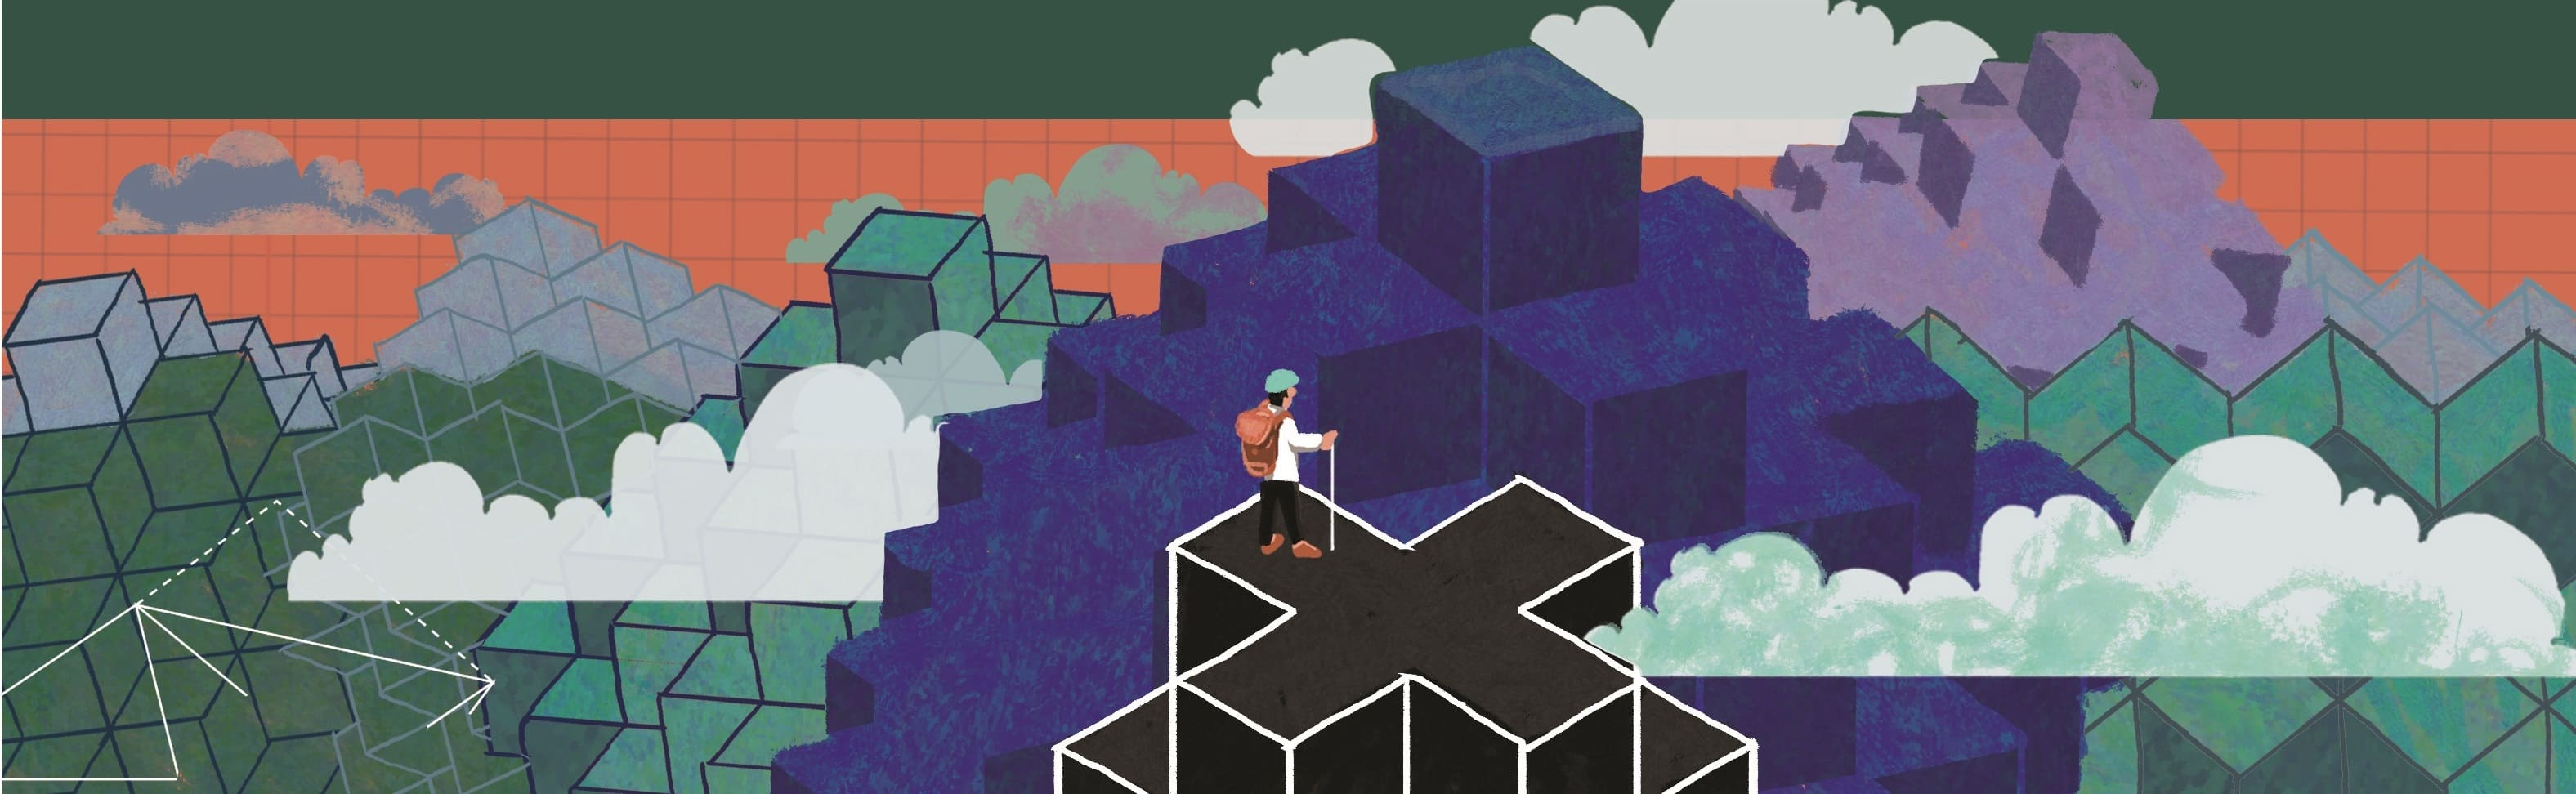
\includegraphics[width=19.3cm]{../thachthuctoanhoc/bannerthachthuc}}}
\centering
\vspace*{4cm}
\endgroup
\vspace*{-8pt}
\begin{tBox}
	\begin{itemize}[leftmargin = 13pt, itemsep = 1.0pt] 
		\item Mỗi bài toán đề xuất (kèm theo lời giải) cần được nêu rõ là bài sáng tác hay bài sưu tầm.
		%		\item Mỗi bài toán đề xuất (kèm theo lời giải) cần được nêu rõ là bài sáng tác hay bài sưu tầm (nếu là bài sưu tầm, cần ghi rõ nguồn).
		\item Bài giải cho mỗi bài toán cần được trình bày trong một file riêng hoặc
		một tờ giấy riêng.
		\item  Người đề xuất bài toán hoặc gửi bài giải cho các bài toán trong mục ``Thách thức kỳ này" cần ghi rõ họ, đệm, tên và nơi làm việc/học tập, số điện thoại liên hệ. Nếu là học sinh (hoặc sinh viên) cần ghi rõ là học sinh lớp mấy (hoặc sinh viên năm thứ mấy).
		\item Các bài toán trong mục Thách thức kỳ này hướng tới các độc giả là học sinh phổ thông; được phân chia thành các mức độ $B$, $A$, và được sắp xếp theo độ khó tăng dần, theo đánh giá chủ quan của Ban biên tập. Các bài toán mức độ $B$ không đòi hỏi các kiến thức vượt quá chương trình môn Toán cấp THCS; các bài toán mức độ $A$ không đòi hỏi các kiến thức vượt quá chương trình môn Toán cấp THPT.
		\item Cách thức gửi bài toán đề xuất hoặc lời giải: gửi file thu được bằng cách scan, ảnh chụp (rõ nét) của bản viết tay, hoặc được soạn thảo bằng các phần mềm Latex, Word tới \url{bbt@pi.edu.vn} hoặc gửi qua đường bưu điện tới Tòa soạn (xem địa chỉ tại bìa $2$).
		\item Hạn gửi lời giải cho các bài toán P$651$--P$660$: trước ngày $15/1/2023$.
	\end{itemize}
\end{tBox}
\begin{center}
	\vspace*{-5pt}
	\textbf{\color{thachthuctoanhoc}\color{thachthuctoanhoc}\color{thachthuctoanhoc}THÁCH THỨC KỲ NÀY}
	\vspace*{-5pt}
\end{center}
\begin{multicols}{2}
	\setlength{\abovedisplayskip}{4pt}
	\setlength{\belowdisplayskip}{4pt}
	{\color{thachthuctoanhoc}{\usefont{T5}{qag}{b}{n} P661.}}
	(Mức $B$) Một xấp tiền giấy có $120$ tờ tiền, gồm các tờ tiền với mệnh giá $10.000$ đồng, $50.000$ đồng, và $100.000$ đồng. Số tờ tiền mệnh giá $50.000$ đồng là một số lớn hơn $5$ và chia hết cho $5$. Hỏi mỗi loại mệnh giá có bao nhiêu tờ tiền? Biết rằng, tổng mệnh giá của cả xấp tiền là $8.600.000$ đồng.
	\begin{flushright}
		\textit{Đăng Hải, Hà Nội}
	\end{flushright}
	{\color{thachthuctoanhoc}{\usefont{T5}{qag}{b}{n} P662.}}
	(Mức $B$) Với mỗi số thực $x$, đặt $f(x)=\sqrt[3]{x^3-x}$. Cho các số thực đôi một phân biệt $a,b,c$ thoả mãn
	\begin{align*}
		&a f(b)+b f(c)+c f(a)\\
		=\,&a f(c)+b f(a)+c f(b)=0.
	\end{align*}
	Chứng minh rằng $a+b+c=0$. 
	\begin{flushright}
		\textit{Phan Quang Đạt, Hà Nội}
	\end{flushright}
	{\color{thachthuctoanhoc}{\usefont{T5}{qag}{b}{n} P663.}}
	(Mức $B$) Cho hai đường tròn đồng tâm $(C_1)$ và $(C_2)$, có bán kính, tương ứng, là $14$ và $50$. Tìm số nguyên dương $k$ nhỏ nhất có tính chất: Nếu qua một điểm tuỳ ý nằm trên $(C_1)$, kẻ $k$ dây cung tuỳ ý của $(C_2)$ thì chắc chắn có một dây cung có độ dài không nguyên. 
	\vskip 0.05cm
	\hfill	\textit{Hà Duy Hưng, Hà Nội}
	\vskip 0.05cm
	{\color{thachthuctoanhoc}{\usefont{T5}{qag}{b}{n} P664.}}
	(Mức $B$) Giải hệ phương trình
	\begin{align*}
		\begin{cases}
			x^{23}=3y^{21}-2z^{19}&\\
			y^{23}=3z^{21}-2x^{19}&\\
			z^{23}=3x^{21}-2y^{19}.
		\end{cases}
	\end{align*}
	\hfill	\textit{Bằng Linh, Phú Thọ}
	\vskip 0.05cm
	{\color{thachthuctoanhoc}{\usefont{T5}{qag}{b}{n} P665.}}
	(Mức $B$) Cho số thực $k\ge1$, và cho tam giác đều $ABC$ cạnh $a$. Một điểm $M$ di động trên đường tròn ngoại tiếp của tam giác đó. Hãy tìm giá trị nhỏ nhất và lớn nhất của biểu thức $S=kMA+MB+MC$.
	\begin{figure}[H]
		\vspace*{-10pt}
		\centering
		\captionsetup{labelformat= empty, justification=centering}
		\definecolor{ffqqqq}{rgb}{1,0,0}
		\definecolor{qqzzcc}{rgb}{0,0.6,0.8}
		\definecolor{qqqqff}{rgb}{0,0,1}
		\definecolor{qqqqffa}{rgb}{1,1,1}
		\definecolor{cqcqcq}{rgb}{0.7529411764705882,0.7529411764705882,0.7529411764705882}
		\begin{tikzpicture}[scale=0.6,node font = \small]
			\draw [color=qqzzcc] (0,3.196152422706632)-- (-3,-2);
			\draw [color=qqzzcc] (-3,-2)-- (3,-2);
			\draw [color=qqzzcc] (3,-2)-- (0,3.196152422706632);
			\draw [,color=ffqqqq] (0,-0.2679491924311226) circle (3.4641016151377544cm);
			\draw [] (1.473281922635266,-3.4031430263808087)-- (3,-2);
			\draw [] (-3,-2)-- (1.473281922635266,-3.4031430263808087);
			\draw [] (1.473281922635266,-3.4031430263808087)-- (0,3.196152422706632);
			\draw [fill=qqqqffa] (-3,-2) circle (1.6pt);
			\draw[color=qqqqff] (-3.38,-2.35) node {$B$};
			\draw [fill=qqqqffa] (3,-2) circle (1.6pt);
			\draw[color=qqqqff] (3.34,-2.27) node {$C$};
			\draw [fill=qqqqffa] (0,3.196152422706632) circle (1.6pt);
			\draw[color=qqqqff] (0,3.75) node {$A$};
			\draw [fill=qqqqffa] (1.473281922635266,-3.4031430263808087) circle (1.6pt);
			\draw[color=qqqqff] (1.65,-3.75) node {$M$};
			\draw [fill=qqqqffa] (0,-0.2679491924311226) circle (1.6pt);
			\draw[color=qqqqff] (-0.4,-0.13) node {$O$};
		\end{tikzpicture}
		\vspace*{-10pt}
	\end{figure}
	\hfill	\textit{Hoàng Ngọc Minh, Hà Nội}
	\vskip 0.1cm
	{\color{thachthuctoanhoc}{\usefont{T5}{qag}{b}{n} P666.}}
	(Mức $B$) Cho số nguyên $n\ge13$. Chứng minh rằng, không thể chia một hình vuông cạnh $n$ thành năm hình chữ nhật, với độ dài các cạnh là $1,2,3,4,5,6,7,8,9,10$, như hình dưới đây.
	\begin{figure}[H]
		\vspace*{-10pt}
		\centering
		\captionsetup{labelformat= empty, justification=centering}
		\definecolor{qqqqff}{rgb}{0,0,1}
		\definecolor{qqqqffa}{rgb}{1,1,1}
		\begin{tikzpicture}[thachthuctoanhoc,scale=0.35]
			\draw [] (-5,5)-- (5,5);
			\draw [] (5,5)-- (5,-5);
			\draw [] (-5,5)-- (-5,-5);
			\draw [] (-5,-5)-- (5,-5);
			\draw [] (-1.8064850795005638,5)-- (-1.806485079500564,-0.9133587450621485);
			\draw [] (-5,-0.9133587450621485)-- (1.4776647785694939,-0.9133587450621485);
			\draw [] (1.4776647785694939,1.1789625354824862)-- (1.477664778569494,-5);
			\draw [] (-1.806485079500564,1.1789625354824862)-- (5,1.1789625354824862);
			\draw [fill=qqqqffa] (-5,5) circle (1.6pt);
			\draw [fill=qqqqffa] (5,5) circle (1.6pt);
			\draw [fill=qqqqffa] (5,-5) circle (1.6pt);
			\draw [fill=qqqqffa] (-5,-5) circle (1.6pt);
			\draw [fill=qqqqffa] (-1.8064850795005638,5) circle (1.6pt);
			\draw [fill=qqqqffa] (5,1.1789625354824862) circle (1.6pt);
			\draw [fill=qqqqffa] (-5,-0.9133587450621485) circle (1.6pt);
			\draw [fill=qqqqffa] (1.477664778569494,-5) circle (1.6pt);
			\draw [fill=qqqqffa] (-1.806485079500564,1.1789625354824862) circle (1.6pt);
			\draw [fill=qqqqffa] (1.4776647785694939,1.1789625354824862) circle (1.6pt);
			\draw [fill=qqqqffa] (1.4776647785694939,-0.9133587450621485) circle (1.6pt);
			\draw [fill=qqqqffa] (-1.806485079500564,-0.9133587450621485) circle (1.6pt);
		\end{tikzpicture}
		\vspace*{-10pt}
	\end{figure}
	\hfill\textit{Phạm Như Ngọc, Hải Phòng}
	\vskip 0.1cm
	{\color{thachthuctoanhoc}{\usefont{T5}{qag}{b}{n} P667.}}
	(Mức $A$) Chứng minh rằng
	\begin{align*}
		8(x+y-1)^2-9xy(x+y-1)+xy\ge0
	\end{align*}
	với mọi $x,y\in[0;1]$. 
	\vskip 0.1cm
		\hfill\textit{Nguyễn Tấn Mạnh và Nguyễn Anh Vũ}, 
		\vskip 0.01cm
		\hfill \textit{Bình Định}
	\vskip 0.1cm
	{\color{thachthuctoanhoc}{\usefont{T5}{qag}{b}{n} P668.}}
	(Mức $A$) Cho số nguyên $n\ge2$. Có $n$ con ếch nằm trên một trục số, tại $n$ điểm tuỳ ý, thuộc tập $2n$ điểm $1,2,\ldots,2n$. Vào cùng một thời điểm, mỗi con ếch đều nhảy đến một trong số $n$ điểm còn lại, thuộc tập $2n$ điểm vừa nêu, sao cho không có hai con nào cùng nhảy tới một điểm. Chứng minh rằng
	\vskip 0.05cm
	$a)$ Tổng khoảng cách $n$ con ếch đã nhảy không vượt quá $n^2$. 
	\vskip 0.05cm
	$b)$ Tồn tại một phương án nhảy của $n$ con ếch, sao cho tổng khoảng cách chúng đã nhảy đúng bằng $n^2$. 
	\vskip 0.1cm
	\hfill	\textit{Lê Vĩ, Hà Nội}
	\vskip 0.1cm
	{\color{thachthuctoanhoc}{\usefont{T5}{qag}{b}{n} P669.}}
	(Mức $A$) Cho tam giác nhọn $ABC$, với $AB<AC$, nội tiếp đường tròn $(O)$. Gọi $M,N$ tương ứng là trung điểm của các cung $BC$ lớn và cung $BC$ nhỏ. Trên đường thẳng $AN$, lấy điểm $D$ sao cho $D$ nằm trong tam giác $ABC$ và không trùng với tâm đường tròn nội tiếp tam giác ấy. Trên đoạn thẳng $MD$, lấy điểm $T$ sao cho $\angle{MBT}=\angle{DCB}$. Chứng minh rằng trực tâm của tam giác $TND$ nằm trên đường thẳng $BC$.
	\begin{figure}[H]
		\vspace*{-10pt}
		\centering
		\captionsetup{labelformat= empty, justification=centering}
		\definecolor{qqwuqq}{rgb}{0,0.39215686274509803,0}
		\definecolor{ffqqqq}{rgb}{1,0,0}
		\definecolor{qqzzff}{rgb}{0,0.6,1}
		\definecolor{qqqqff}{rgb}{0,0,1}
		\definecolor{qqqqffa}{rgb}{1,1,1}
		\begin{tikzpicture}[scale=0.5,node font = \small]
			\draw [shift={(-4.52,-2)},color=qqwuqq] (0,0) -- (44.80816980779454:0.9) arc (44.80816980779454:59.48716265964927:0.9) -- cycle;
			\draw [shift={(3,-2)},,color=qqwuqq] (0,0) -- (165.3210071481453:0.9) arc (165.3210071481453:180:0.9) -- cycle;
			\draw [color=qqzzff] (-3.08,3.7)-- (-4.52,-2);
			\draw [color=qqzzff] (-4.52,-2)-- (3,-2);
			\draw [color=qqzzff] (3,-2)-- (-3.08,3.7);
			\draw [color=ffqqqq] (-0.76,0.082) circle (4.297944159711711cm);
			\draw [] (-3.08,3.7)-- (-0.76,-4.215944159711711);
			\draw [] (-1.7761254755175533,-0.7488784168421159)-- (3,-2);
			\draw [] (-4.52,-2)-- (-0.76,4.379944159711711);
			\draw [] (-4.52,-2)-- (-1.4124345691125013,1.0868261064673503);
			\draw [] (-1.7761254755175533,-0.7488784168421159)-- (-0.76,4.379944159711711);
			\draw [] (-1.4124345691125013,1.0868261064673503)-- (-0.76,-4.215944159711711);
			\draw [shift={(-4.52,-2)},,color=qqwuqq] (44.80816980779454:0.9) arc (44.80816980779454:59.48716265964927:0.9);
			\draw[,color=qqwuqq] (-4.0045520409083055,-1.3367403212404605) -- (-3.9309166181809205,-1.241988938560526);
			\draw [shift={(3,-2)},,color=qqwuqq] (165.3210071481453:0.9) arc (165.3210071481453:180:0.9);
			\draw[,color=qqwuqq] (2.1668824426700812,-1.8926913998384574) -- (2.0478656487658085,-1.8773615998153805);
			\draw [fill=qqqqffa] (-3.08,3.7) circle (1.6pt);
			\draw[color=qqqqff] (-3.2,4.19) node {$A$};
			\draw [fill=qqqqffa] (-4.52,-2) circle (1.6pt);
			\draw[color=qqqqff] (-4.99,-2.19) node {$B$};
			\draw [fill=qqqqffa] (3,-2) circle (1.6pt);
			\draw[color=qqqqff] (3.44,-2.29) node {$C$};
			\draw [fill=qqqqffa] (-0.76,4.379944159711711) circle (1.6pt);
			\draw[color=qqqqff] (-0.82,4.81) node {$M$};
			\draw [fill=qqqqffa] (-0.76,-4.215944159711711) circle (1.6pt);
			\draw[color=qqqqff] (-0.8,-4.7) node {$N$};
			\draw [fill=qqqqffa] (-1.7761254755175533,-0.7488784168421159) circle (1.6pt);
			\draw[color=qqqqff] (-2.2,-0.95) node {$D$};
			\draw [fill=qqqqffa] (-1.4124345691125013,1.0868261064673503) circle (1.6pt);
			\draw[color=qqqqff] (-1,1.1) node {$T$};
		\end{tikzpicture}
		\vspace*{-10pt}
	\end{figure}
	\hfill\textit{Đỗ Đại Phong, Thừa Thiên Huế}
	\vskip 0.1cm
	{\color{thachthuctoanhoc}{\usefont{T5}{qag}{b}{n} P670.}}
	(Mức $A$) Hỏi, có thể chọn được tối đa bao nhiêu điểm nguyên trong mặt phẳng toạ độ, sao cho đoạn thẳng nối hai điểm bất kỳ trong chúng chứa đúng $2022$ điểm nguyên?
	\vskip 0.05cm
	(Trong mặt phẳng toạ độ, một điểm được gọi là {\it điểm nguyên}, nếu cả hoành độ và tung độ của nó đều là các số nguyên.)
	\vskip 0.1cm
	\hfill	\textit{Nguyễn Thành Khang, Hà Nội}
\end{multicols}
\centerline{{\large{\textbf{\color{thachthuctoanhoc}GIẢI BÀI KỲ TRƯỚC}}}}
\vspace*{-5pt}
\begin{multicols}{2}
	\setlength{\abovedisplayskip}{4pt}
	\setlength{\belowdisplayskip}{4pt}
	{\color{thachthuctoanhoc}{\usefont{T5}{qag}{b}{n} P631.}}
	(Mức $B$) Các số tự nhiên, bắt đầu từ $20$, được viết liên tiếp nhau thành một hàng ngang, như sau:
	\vskip 0.05cm
	\columnbreak
	\centerline{$2021222324252627\ldots.$}
	Hỏi chữ số ở vị trí thứ $2022$, kể từ trái qua phải, là chữ số nào?
	\vskip 0.05cm
	\textbf{\color{thachthuctoanhoc}Lời giải} (\textit{của bạn Võ Trần Tiến, lớp $8^5$, trường THCS Long Bình Điền, tỉnh Tiền Giang})\textbf{\color{thachthuctoanhoc}.}
	\vskip 0.05cm
	Gọi $a$ là chữ số ở vị trí thứ $2022$, kể từ trái qua phải.
	\vskip 0.05cm
	Nhận thấy:
	\vskip 0.05cm
	-- Từ $20$ đến $99$ có $(99-20 + 1) \cdot 2 = 160$ chữ số;
	\vskip 0.05cm
	-- Từ $100$ đến $999$ có  $(999 -100+1)\cdot 3 = 2700$ chữ số.
	\vskip 0.05cm
	Vì $160 < 2022 < 160 + 2700$ nên $a$ là chữ số của một số tự nhiên có ba chữ số.
	\vskip 0.05cm
	Từ đó, do
	\begin{align*}
		2022 - 160 = 3 \cdot 620 + 2
	\end{align*}
	nên $a$ là chữ số thứ hai (kể từ trái qua phải) của số tự nhiên có ba chữ số thứ $621$.
	\vskip 0.05cm
	Số tự nhiên có ba chữ số thứ $621$ là:
	\begin{align*}
		100 + 621 - 1 = 720.
	\end{align*}
	Vì vậy, $a$ là chữ số $2$.
	\vskip 0.05cm
	Ta có điều phải tìm theo yêu cầu đề bài.
	\vskip 0.05cm
	\textbf{\color{thachthuctoanhoc}Bình luận và Nhận xét}
	\vskip 0.05cm	
	Tất cả các lời giải Tạp chí đã nhận được từ bạn đọc đều là lời giải đúng và hoàn chỉnh.
	\begin{flushright}
		\textbf{\color{thachthuctoanhoc}Hà Thanh}
	\end{flushright}
	{\color{thachthuctoanhoc}{\usefont{T5}{qag}{b}{n} P632.}}
	(Mức $B$) Cho $x,y,z$ là các số thực dương thoả mãn 
	\begin{align*}
		\dfrac{x^2}{(x+y)^2}+\dfrac{y^2}{(y+z)^2}+\dfrac z{z+x}=1.
	\end{align*}
	Chứng minh rằng $x=y=z$. 
	\vskip 0.05cm
	\textbf{\color{thachthuctoanhoc}Lời giải.}
	Do $x, y, z > 0$ nên hệ thức của đề bài tương đương với
	\begin{align*}
		\frac{1}{{{{\left( {1 + \frac{y}{x}} \right)}^2}}} + \frac{1}{{{{\left( {1 + \frac{z}{y}} \right)}^2}}} = \frac{1}{{1 + \frac{z}{x}}}.\tag{$1$}
	\end{align*}
	Đặt $a = \dfrac{y}{x}$  và  $b = \dfrac{z}{y}$, ta có $a, b > 0$, và ($1$) được viết lại dưới dạng:
	\begin{align*}
		\frac{1}{{{{\left( {1 + a} \right)}^2}}} + \frac{1}{{{{\left( {1 + b} \right)}^2}}} = \frac{1}{{1 + ab}}.\tag{$2$}
	\end{align*}
	Tiếp theo, có thể giải bài toán theo một trong hai cách sau:
	\vskip 0.05cm
	\columnbreak
	$\bullet$ \textbf{\color{thachthuctoanhoc}Cách} $\pmb{1}$ (\textit{của người đề xuất bài toán})\textbf{\color{thachthuctoanhoc}.}
	\vskip 0.05cm
	Ta có:
	\begin{align*}
		(2)\!\Leftrightarrow &{\left( {\frac{1}{{1 + a}} - \frac{1}{{1 + b}}} \right)^2} \\[-0.4ex]
		&= \frac{1}{{1 + ab}} - \frac{2}{{\left( {1 + a} \right)\left( {1 + b} \right)}}\\[-0.4ex]
		\Leftrightarrow &\frac{{{{\left( {a - b} \right)}^2}}}{{{{\left(\!{1 \!+\! a}\! \right)}^2}\!{{\left( \!{1 + b}\! \right)}^2}}} \!=\! \frac{{a + b - ab - 1}}{{\left(\! {1 \!+\! ab}\! \right)\!\left(\! {1 \!+\! a}\! \right)\!\left(\! {1 + b}\! \right)}}\\[-0.4ex]
		\Leftrightarrow&\, \frac{{{{\left( {a - b} \right)}^2}}}{{\left( {1 + a} \right)\left( {1 + b} \right)}}= \frac{{ - \left( {1 - a} \right)\left( {1 - b} \right)}}{{1 + ab}}\\[-0.4ex]
		\Leftrightarrow &\left( {1 \!+\! ab} \right)\!{\left( {a \!-\! b} \right)^2} \!+\! \left(\!\! {1 \!-\! {a^2}} \right)\!\!\left(\!\! {1 \!-\! {b^2}} \right) \!=\! 0\\[-0.4ex]
		\Leftrightarrow &\,\,ab{\left( {a - b} \right)^2} + {\left( {ab - 1} \right)^2} = 0\\[-0.4ex]
		\Leftrightarrow &\,{\left( {a - b} \right)^2} = {\left( {ab - 1} \right)^2} = 0 \text{ (do $ab>0$)}\\[-0.4ex]
		\Leftrightarrow &\,\,a = b = 1.
	\end{align*} 
	Vì vậy
	\begin{align*}
		(1) \Leftrightarrow \frac{y}{x} = \frac{z}{y} = 1 \Leftrightarrow x = y =z.
	\end{align*}
	Ta có điều phải chứng minh theo yêu cầu đề bài.
	\vskip 0.05cm
	$\bullet$ Cách $2$ (\textit{của người chấm bài})\textbf{\color{thachthuctoanhoc}.}
	\vskip 0.05cm
	Do $a, b > 0$ nên áp dụng bất đẳng thức Cauchy -- Schwarz cho hai bộ số  $(1,\sqrt{ab})$ và  $\left(1, \sqrt{\dfrac{a}{b}}\right)$, ta được:
	\begin{align*}
		&\frac{1}{{{{\left( {1 + a} \right)}^2}}} = \frac{1}{{{{\left( {1 \cdot 1 + \sqrt {ab}  \cdot \sqrt {\frac{a}{b}} } \right)}^2}}} \\[-0.4ex]
		\ge &\frac{1}{{\left( {1 + ab} \right)\left( {1 + \frac{a}{b}} \right)}}= \frac{b}{{\left( {1 + ab} \right)\left( {b + a} \right)}};
	\end{align*}
	đẳng thức xảy ra khi và chỉ khi $b = 1$.
	\vskip 0.05cm
	Bằng cách hoàn toàn tương tự, ta có:
	\begin{align*}
		\frac{1}{{{{\left( {1 + b} \right)}^2}}} \ge \frac{a}{{\left( {1 + ab} \right)\left( {a + b} \right)}};
	\end{align*}
	đẳng thức xảy ra khi và chỉ khi $a = 1$.
	\vskip 0.05cm
	Do đó
	\begin{align*}
		&\frac{1}{{{{\left( {1 + a} \right)}^2}}} + \frac{1}{{{{\left( {1 + b} \right)}^2}}} \\[-0.4ex]
		\ge &\frac{b}{{\left( {1 + ab} \right)\left( {b + a} \right)}} + \frac{a}{{\left( {1 + ab} \right)\left( {a + b} \right)}} \\[-0.4ex]
		= &\frac{1}{{1 + ab}};
	\end{align*}
	đẳng thức xảy ra khi và chỉ khi $b = a = 1$.
	\vskip 0.05cm
	Vì thế, $(2) \Leftrightarrow b = a = 1$; hay
	\begin{align*}
		(1)  \Leftrightarrow  \dfrac{z}{y} = \dfrac{y}{x} = 1  \Leftrightarrow  x = y = z.
	\end{align*}
	Ta có điều phải chứng minh theo yêu cầu đề bài.
	\vskip 0.05cm
	\textbf{\color{thachthuctoanhoc}Bình luận và Nhận xét}
	\vskip 0.05cm
	$\pmb{1.}$ Trong số các lời giải Tạp chí đã nhận được từ bạn đọc, rất tiếc, có một số lời giải không được chấp nhận là lời giải đúng, do người giải bài đã mắc một trong các lỗi sau:
	\vskip 0.05cm
	-- \textit{Ngộ nhận} rằng, nếu $a, b, c > 0$ và $abc = 1$, thì
	\begin{align*}
		\frac{1}{{{{\left( {1 \!+\! a} \right)}^2}}} \!+\! \frac{1}{{{{\left( {1 \!+\! b} \right)}^2}}} \!+\! \frac{1}{{1 \!+\! c}} \!=\! 1 \!\Leftrightarrow\! a \!=\!b \!=\!c.
	\end{align*}
	-- Mới chỉ chứng minh được rằng, nếu $x, y, z > 0$ thì
	\begin{align*}
		\frac{{{x^2}}}{{{{\left( {x + y} \right)}^2}}} + \frac{{{y^2}}}{{{{\left( {y + z} \right)}^2}}} + \frac{z}{{z + x}} \ge 1.
	\end{align*}
	-- Đưa ra lời giải cho một bài toán, \textit{khác với bài đã ra}: ``Hệ thức ở bài đã ra xảy ra \textit{khi} $x = y = z$".
	\vskip 0.05cm
	$\pmb{2.}$ Bên cạnh các lời giải không đúng nêu trên, có một số lời giải không được coi là hoàn chỉnh, do người giải bài đã mắc các lỗi ``chính tả" không thể châm chước; chẳng hạn như:
	\begin{align*}
		\frac{y}{x} = \frac{z}{y} = 1 \Leftrightarrow  x = y = z = 1.
	\end{align*}
	\hfill	\textbf{\color{thachthuctoanhoc}Lê Huy}
	\vskip 0.1cm
	{\color{thachthuctoanhoc}{\usefont{T5}{qag}{b}{n} P633.}}
	(Mức $B$) Chứng minh rằng, với mọi số nguyên dương $n$, số dư trong phép chia số $A=n^{2024}+n^{2025}$  cho số $B=n+n^2+n^3+\cdots+n^{2022}$ là một số chẵn. 
	\vskip 0.05cm
	\textbf{\color{thachthuctoanhoc}Lời giải} (\textit{phỏng theo ý giải của bạn Ngô Quang Bình, lớp $11$T$1$, trường THPT chuyên Lê Hồng Phong, tỉnh Nam Định})\textbf{\color{thachthuctoanhoc}.}
	\vskip 0.05cm
	Từ giả thiết của bài ra, ta có:
	\begin{align*}
		A = \,\,&{n^{2024}}\left( {1 + n} \right), \tag{$1$}\\
		B = \,\,&n\left( {1 + n} \right) + {n^3}\left( {1 + n} \right) +  \cdots  \\
		&+ {n^{2021}}\left( {1 + n} \right). \tag{$2$}
	\end{align*}
	Gọi $q$ và $r$ tương ứng là thương và số dư trong phép chia $A$ cho $B$, ta có:
	\begin{align*}
		A = Bq + r. \tag{$3$}
	\end{align*}
	Vì với mọi số nguyên dương $n, n(n + 1)$ là một số chẵn, nên từ ($1$) và ($2$) suy ra, với mọi số nguyên dương $n$, $A$ và $B$ là các số chẵn. Vì thế, từ ($3$) suy ra, với mọi số nguyên dương $n$, $r$ là một số chẵn.
	\vskip 0.05cm
	Ta có điều phải chứng minh theo yêu cầu đề bài.
	\vskip 0.05cm
	\textbf{\color{thachthuctoanhoc}Bình luận và Nhận xét}
	\vskip 0.05cm
	$\pmb{1.}$ Trong số các lời giải Tạp chí đã nhận được từ bạn đọc, rất tiếc, có một số lời giải sai, do người giải bài đã mắc một trong các lỗi dưới đây:
	\vskip 0.05cm
	-- \textit{Xác định sai số dư} trong phép chia $A$ cho $B$;
	\vskip 0.05cm
	--\textit{ Ngộ nhận rằng, $B = \frac{{{n^{2023}} - 1}}{{n - 1}}$  với mọi} $n \in \mathbb{N^*}$  và đồng thời, \textit{chưa đi đến điều phải chứng minh} theo yêu cầu đề bài.
	\vskip 0.05cm
	(\textit{\textbf{\color{thachthuctoanhoc}Lưu ý}: Với $a$, $b$, $m$ là các số nguyên dương, $m > 1$, đồng dư thức $a \equiv b\left( {\bmod m} \right)$  \textbf{\color{thachthuctoanhoc}không} tương đương với ``$b$ là số dư trong phép chia $a$ cho $m$".})
	\vskip 0.05cm
	$\pmb{2.}$ Bên cạnh các lời giải sai nêu trên, có một lời giải không được coi là lời giải hoàn chỉnh, do người giải bài chứng minh thiếu chặt chẽ, thiếu chính xác sự kiện $n^2 + n^3$  là số dư trong phép chia $A$ cho $B$.
	\vskip 0.05cm
	$\pmb{3.}$ Với các giả thiết của bài ra, có thể chứng minh được rằng, thương số trong phép chia $A$ cho $B$ là một số tự nhiên chia hết cho $6$.
	\vskip 0.15cm
	\hfill	\textbf{\color{thachthuctoanhoc}Lưu Thị Thanh Hà}
	\vskip 0.15cm
	{\color{thachthuctoanhoc}{\usefont{T5}{qag}{b}{n} P634.}}
	(Mức $B$) Bạn Pi ghi số $4$ vào hình tròn nhỏ, nằm ở tâm của đường tròn lớn trong Hình dưới đây. Sau đó, Pi muốn ghi tiếp vào mỗi hình tròn nhỏ còn lại một số nguyên, sao cho hai điều kiện sau được đồng thời thoả mãn: 
	\vskip 0.05cm
	$i)$ Tổng của tám số ở tám hình tròn nhỏ nằm trên đường tròn lớn bằng $66$. 
	\vskip 0.05cm
	$ii)$ Tổng của ba số ở ba hình tròn nhỏ, nằm trên cùng một đường kính của đường tròn lớn, đều bằng nhau. 
	\vskip 0.05cm
	Hỏi, Pi có thể thực hiện được ý muốn của mình hay không? Vì sao?
	\begin{figure}[H]
		\centering
		\vspace*{-10pt}
		\captionsetup{labelformat= empty, justification=centering}
		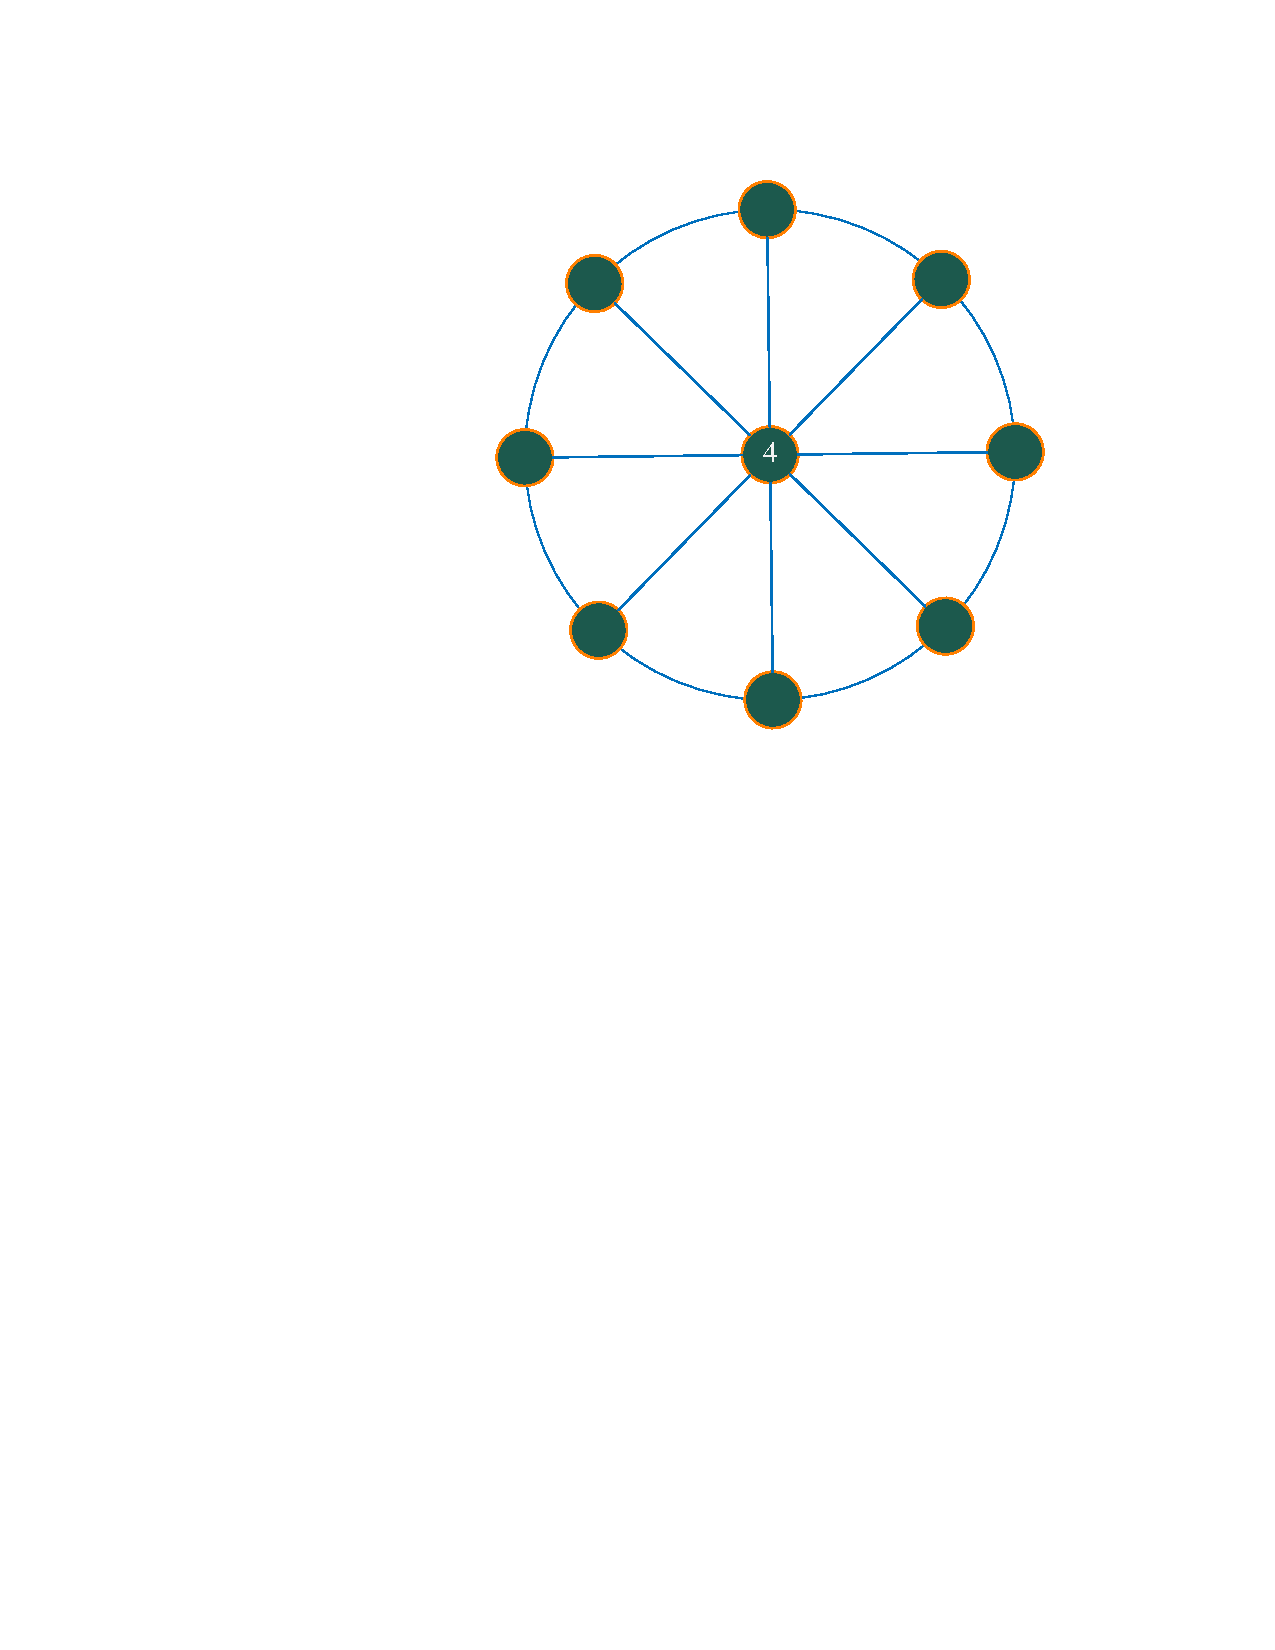
\includegraphics[width=0.65\linewidth]{P634}
		\vspace*{-10pt}
	\end{figure}
	\textbf{\color{thachthuctoanhoc}Lời giải} (\textit{dựa theo tất cả lời giải Tạp chí đã nhận được từ bạn đọc})\textbf{\color{thachthuctoanhoc}.}
	\vskip 0.05cm
	Giả sử Pi thực hiện được ý muốn của mình.
	\vskip 0.05cm
	Xét một cách điền bất kỳ của Pi, thỏa mãn các điều kiện $i)$ và $ii)$.
	\vskip 0.05cm
	Gọi $S$ là tổng của tám số ở tám hình tròn nhỏ, nằm trên đường tròn lớn. Theo $i)$, \linebreak $S = 66$.       \hfill              ($1$)
	\vskip 0.05cm
	Gọi $s$ là tổng của ba số ở ba hình tròn nhỏ, nằm trên cùng một đường kính tùy ý của đường tròn lớn. Do các số ở các hình tròn nhỏ là các số nguyên, nên $s$ là một số nguyên.
	\vskip 0.05cm
	Theo $ii)$, tổng của ba số ở ba hình tròn nhỏ, nằm trên mỗi đường kính, trong số ba đường kính còn lại của đường tròn lớn, cũng bằng $s$. Vì thế, từ quan sát hình đã cho ở đề bài, ta có:
	\begin{align*}
		4s = 4 \cdot 4 + S. \tag{$2$}
	\end{align*}
	Từ ($1$) và ($2$), suy ra $4s = 82$. Từ đây, vì $s$ là số nguyên nên $82$ chia hết cho $4$, là điều vô lý.
	\vskip 0.05cm
	Điều vô lý nhận được ở trên cho thấy, giả sử ở đầu lời giải là sai; nghĩa là, Pi \textit{không thể} thực hiện được ý muốn của mình.
	\vskip 0.05cm
	\textbf{\color{thachthuctoanhoc}Bình luận và Nhận xét}
	\vskip 0.05cm
	Tất cả lời giải Tạp chí đã nhận được từ bạn đọc đều là lời giải đúng và hoàn chỉnh.
	\vskip 0.15cm
	\hfill	\textbf{\color{thachthuctoanhoc}Nguyễn Khắc Minh}
	\vskip 0.15cm
	{\color{thachthuctoanhoc}{\usefont{T5}{qag}{b}{n} P635.}}
	(Mức $B$) Chứng minh rằng, với mọi số nguyên $n\ge2$, ta luôn có:
	\begin{align*}
		\dfrac{1}{2!}+\dfrac{2}{3!}+\ldots+\dfrac{2^{n-2}}{n!}\le\dfrac{3}{2}.
	\end{align*}
	(Với mỗi số nguyên dương $k$, $k!$ (đọc là, ``$k$ giai thừa") ký hiệu tích của $k$ số nguyên dương đầu tiên; tức là, $k!=1\cdot2\cdots k$.)
	\vskip 0.05cm
	\textbf{\color{thachthuctoanhoc}Lời giải} (\textit{phỏng theo ý giải của bạn Nguyễn Công Minh Đức, lớp $11$ Toán $1$, trường THPT chuyên Hưng Yên, tỉnh Hưng Yên})\textbf{\color{thachthuctoanhoc}.}
	\vskip 0.05cm
	Trước hết, ta chứng minh Nhận xét sau:
	\vskip 0.05cm
	\textbf{\color{thachthuctoanhoc}Nhận xét.} Với mọi số nguyên $k \ge 3$, ta có:
	\begin{align*}
		\frac{{{2^{k - 2}}}}{{k!}} \le 2\left( {\frac{1}{{k - 1}} - \frac{1}{k}} \right).
	\end{align*}
	\textit{Chứng minh.} Dễ thấy, bất đẳng thức cần chứng minh tương đương với bất đẳng thức
	\begin{align*}
		{2^{k - 3}} \le \left( {k - 2} \right)!. \tag{$*$}
	\end{align*}
	Với $k = 3$, hiển nhiên ($*$) là một bất đẳng thức đúng.
	\vskip 0.05cm
	Xét $k \ge 4$. Khi đó, $k - 2 \ge 2$. Do đó
	\begin{align*}
		\left( {k - 2} \right)! &= \left( {k - 2} \right)\left( {k - 3} \right) \cdots 2 \\
		&\ge \underbrace {2 \cdot 2 \cdot  \cdots  \cdot 2}_{k - 3\text{ thừa số }2} = {2^{k - 3}}.
	\end{align*}
	Bất đẳng thức ($*$) được chứng minh, và do đó, bất đẳng thức của Nhận xét được chứng minh.
	\vskip 0.05cm
	\textit{Trở lại bài toán.}
	\vskip 0.05cm
	Dễ thấy, với $n = 2$, bất đẳng thức của đề bài là một bất đẳng thức đúng.
	\vskip 0.05cm
	Xét $n \ge 3$. Khi đó, theo Nhận xét trên, ta có:
	\begin{align*}
		&\frac{1}{{2!}} + \frac{2}{{3!}} + \frac{{{2^2}}}{{4!}} +  \cdots  + \frac{{{2^{n - 2}}}}{{n!}} \\
		\le &\frac{1}{2} + 2\left( \left( {\frac{1}{2} - \frac{1}{3}} \right) + \left( {\frac{1}{3} - \frac{1}{4}} \right) +  \cdots \right. \\
		&\left.+ \left( {\frac{1}{{n - 1}} - \frac{1}{n}} \right) \right)\\
		= &\frac{1}{2} + 2\left( {\frac{1}{2} - \frac{1}{n}} \right) = \frac{3}{2} - \frac{2}{n} < \frac{3}{2}.
	\end{align*}
	Vì vậy, bất đẳng thức của đề bài được chứng minh.
	\vskip 0.05cm
	\columnbreak
	\textbf{\color{thachthuctoanhoc}Bình luận và Nhận xét}
	\vskip 0.05cm
	Trong số các lời giải Tạp chí đã nhận được từ bạn đọc, rất tiếc, có hai lời giải không được chấp nhận là lời giải hoàn chỉnh, do người giải bài không chứng minh các đánh giá mang tính ``chìa khóa" trong lời giải.
	\vskip 0.1cm
	\hfill	\textbf{\color{thachthuctoanhoc}Lê Huy}
	\vskip 0.1cm
	{\color{thachthuctoanhoc}{\usefont{T5}{qag}{b}{n} P636.}}
	(Mức $B$) Cho tam giác nhọn $ABC$, nội tiếp đường tròn $(O)$. Xét lục giác lồi $MNPQRS$ có các đỉnh $M, N$ thuộc cạnh $BC$, các đỉnh $P, Q$ thuộc cạnh $CA$, các đỉnh $R, S$ thuộc cạnh $AB$, sao cho
	\begin{align*}
		\angle{ROQ} &=\angle{BAC},\; \angle{MOS} =\angle{CBA}\;\\
		&\text{\color{black}và}\;\angle{NOP }= \angle{ACB}.
	\end{align*}
	Chứng minh rằng 
	\begin{align*}
		MN + PQ + RS \leq NP + QR + SM.
	\end{align*}
	\textbf{\color{thachthuctoanhoc}Lời giải} (\textit{của bạn Trần Minh Hoàng, lớp $10$T$1$, trường THPT chuyên Hà Tĩnh, tỉnh Hà Tĩnh})\textbf{\color{thachthuctoanhoc}.}
	\begin{figure}[H]
		\centering
		\vspace*{-10pt}
		\captionsetup{labelformat= empty, justification=centering}
		\definecolor{qqwuqq}{rgb}{0.,0.39215686274509803,0.}
		\definecolor{uuuuuu}{rgb}{0.26666666666666666,0.26666666666666666,0.26666666666666666}
		\definecolor{ffqqqq}{rgb}{1.,0.,0.}
		\definecolor{xdxdff}{rgb}{0.49019607843137253,0.49019607843137253,1.}
		\definecolor{qqqqff}{rgb}{0.,0.,1.}
		\begin{tikzpicture}[scale=0.6,node font= \small]
			\draw [shift={(2.1249983220271007,1.0078498119199826)},,pattern color=qqwuqq,fill=qqwuqq,fill opacity=0.10000000149011612] (0,0) -- (-0.22029171081020696:0.4) arc (-0.22029171081020696:59.198829064869955:0.4) -- cycle;
			\draw [shift={(6.,2.)},,pattern color=qqwuqq,fill=qqwuqq,fill opacity=0.10000000149011612] (0,0) -- (169.1110677998218:0.4) arc (169.1110677998218:228.530188575502:0.4) -- cycle;
			\draw [shift={(6.,2.)},,pattern color=qqwuqq,fill=qqwuqq,fill opacity=0.10000000149011612] (0,0) -- (169.1110677998218:0.8) arc (169.1110677998218:194.3614146618134:0.8) -- cycle;
			\draw [shift={(6.,2.)},,pattern color=qqwuqq,fill=qqwuqq,fill opacity=0.10000000149011612] (0,0) -- (143.8607209378302:0.6) arc (143.8607209378302:169.1110677998218:0.6) -- cycle;
			\draw [shift={(6.,2.)},,pattern color=qqwuqq,fill=qqwuqq,fill opacity=0.10000000149011612] (0,0) -- (-165.63858533818663:0.8) arc (-165.63858533818663:-131.46981142449806:0.8) -- cycle;
			\draw [shift={(6.,2.)},,pattern color=qqwuqq,fill=qqwuqq,fill opacity=0.10000000149011612] (0,0) -- (-131.46981142449806:0.6) arc (-131.46981142449806:-97.30103751080952:0.6) -- cycle;
			\draw [shift={(6.,2.)},,pattern color=qqwuqq,fill=qqwuqq,fill opacity=0.10000000149011612] (0,0) -- (-14.801998083433794:0.6) arc (-14.801998083433794:104.0362434679265:0.6) -- cycle;
			\draw [] (6.,2.) circle (4.cm);
			\draw [,color=ffqqqq] (5.029857499854668,5.8805700005813275)-- (9.86725791928902,0.9780821042293271);
			\draw [] (5.029857499854668,5.8805700005813275)-- (2.769656915559922,4.359000541926636);
			\draw [,color=ffqqqq] (2.7696569155599233,4.359000541926637)-- (5.4916697208604015,-1.9675685661762485);
			\draw [] (2.1249983220271007,1.0078498119199826)-- (2.769656915559922,4.359000541926636);
			\draw [] (2.1249983220271007,1.0078498119199826)-- (5.4916697208604015,-1.9675685661762485);
			\draw (4.82,6.7) node[anchor=north west] {$A$};
			\draw (1.5,1.3) node[anchor=north west] {$B$};
			\draw (9.96,1.34) node[anchor=north west] {$C$};
			\draw [,color=qqqqff] (2.769656915559922,4.359000541926636)-- (3.054282279087836,2.566665720495411);
			\draw [,color=qqqqff] (2.9953665458938055,3.5115152528700584) -- (2.817594113369974,3.483284733311256);
			\draw [,color=qqqqff] (3.006345081277784,3.442381529110791) -- (2.8285726487539526,3.414151009551988);
			\draw [,color=qqqqff] (3.054282279087836,2.566665720495411)-- (5.112997902173607,0.9963614477074136);
			\draw [,color=qqqqff] (5.112997902173607,0.9963614477074136)-- (5.4916697208604015,-1.9675685661762485);
			\draw [,color=qqqqff] (5.382737068533431,-0.4047622562937149) -- (5.20418836232428,-0.4275736462346676);
			\draw [,color=qqqqff] (5.391608164621579,-0.4741978642639403) -- (5.213059458412428,-0.497009254204893);
			\draw [,color=qqqqff] (5.4004792607097265,-0.5436334722341657) -- (5.221930554500576,-0.5664448621751185);
			\draw [] (4.020312072968017,4.187120479685714)-- (7.151414984062024,3.730466848905957);
			\draw [] (7.320568549934373,0.9878737036679017)-- (8.521733569981919,2.341710554382787);
			\draw [] (6.,2.)-- (5.112997902173607,0.9963614477074136);
			\draw [] (6.,2.)-- (7.320568549934373,0.9878737036679017);
			\draw [] (6.,2.)-- (8.521733569981919,2.341710554382787);
			\draw [] (6.,2.)-- (7.151414984062024,3.730466848905957);
			\draw [] (6.,2.)-- (3.054282279087836,2.566665720495411);
			\draw [] (6.,2.)-- (2.1249983220271007,1.0078498119199826);
			\draw [] (6.,2.)-- (5.4916697208604015,-1.9675685661762485);
			\draw [] (6.,2.)-- (2.769656915559922,4.359000541926636);
			\draw [] (6.,2.)-- (4.020312072968017,4.187120479685714);
			\draw [] (6.,2.)-- (5.029857499854668,5.8805700005813275);
			\draw [] (6.,2.)-- (9.86725791928902,0.9780821042293271);
			\draw (4.3,1.) node[anchor=north west] {$M$};
			\draw (7.06,1.0) node[anchor=north west] {$N$};
			\draw (8.52,3.02) node[anchor=north west] {$P$};
			\draw (7.16,4.36) node[anchor=north west] {$Q$};
			\draw (3.52,4.94) node[anchor=north west] {$R$};
			\draw (2.44,3.14) node[anchor=north west] {$S$};
			\draw (5.75,1.9) node[anchor=north west] {$O$};
			\draw (2.3,5.06) node[anchor=north west] {$Y$};
			\draw (5.1,-1.95) node[anchor=north west] {$X$};
			\draw [,color=qqqqff] (3.054282279087836,2.566665720495411)-- (2.1249983220271007,1.0078498119199826);
			\draw [,color=qqqqff] (2.6848678641309616,1.7712355586239625) -- (2.5302569663172276,1.863406434052327);
			\draw [,color=qqqqff] (2.6490236347977087,1.711109098363066) -- (2.494412736983975,1.8032799737914305);
			\draw [] (3.054282279087836,2.566665720495411)-- (4.020312072968017,4.187120479685714);
			\draw [] (4.020312072968017,4.187120479685714)-- (5.029857499854668,5.8805700005813275);
			\draw [,color=qqqqff] (2.1249983220271007,1.0078498119199826)-- (5.112997902173607,0.9963614477074136);
			\draw [,color=qqqqff] (3.5493446620485978,1.0923741010308827) -- (3.5486525969333607,0.9123754314639203);
			\draw [,color=qqqqff] (3.619344144657972,1.0921049645971792) -- (3.618652079542735,0.912106295030217);
			\draw [,color=qqqqff] (3.6893436272673457,1.091835828163476) -- (3.6886515621521085,0.9118371585965136);
			\draw [] (5.112997902173607,0.9963614477074136)-- (7.320568549934373,0.9878737036679017);
			\draw [] (7.320568549934373,0.9878737036679017)-- (9.86725791928902,0.9780821042293271);
			\draw [shift={(6.,2.)},,color=qqwuqq] (169.1110677998218:0.8) arc (169.1110677998218:194.3614146618134:0.8);
			\draw[,color=qqwuqq] (5.2603397373977145,1.97757911850266) -- (5.140394829948694,1.9739432998814699);
			\draw [shift={(6.,2.)},,color=qqwuqq] (143.8607209378302:0.6) arc (143.8607209378302:169.1110677998218:0.6);
			\draw[,color=qqwuqq] (5.504840585513648,2.2154464068986366) -- (5.394805160072236,2.2633233862094446);
			\draw [shift={(6.,2.)},,color=qqwuqq] (-165.63858533818663:0.8) arc (-165.63858533818663:-131.46981142449806:0.8);
			\draw[,color=qqwuqq] (5.392811956659965,1.5770074704857064) -- (5.294349030712932,1.5084140873212266);
			\draw[,color=qqwuqq] (5.346794244564377,1.6522612459535508) -- (5.240868986926167,1.595871177729802);
			\draw [shift={(6.,2.)},,color=qqwuqq] (-131.46981142449806:0.6) arc (-131.46981142449806:-97.30103751080952:0.6);
			\draw[,color=qqwuqq] (5.806758084005368,1.4957604122019723) -- (5.7638154360065625,1.383707170469077);
			\draw[,color=qqwuqq] (5.748132023868733,1.522336391799061) -- (5.69216136250623,1.416188923309963);
			\draw [shift={(6.,2.)},,color=qqwuqq] (-14.801998083433794:0.6) arc (-14.801998083433794:104.0362434679265:0.6);
			\draw [shift={(6.,2.)},,color=qqwuqq] (-14.801998083433794:0.5) arc (-14.801998083433794:104.0362434679265:0.5);
			\draw [fill=qqqqff] (6.,2.) circle (1.5pt);
			\draw [fill=xdxdff] (5.029857499854668,5.8805700005813275) circle (1.5pt);
			\draw [fill=xdxdff] (9.86725791928902,0.9780821042293271) circle (1.5pt);
			\draw [fill=xdxdff] (2.769656915559922,4.359000541926636) circle (1.5pt);
			\draw [fill=xdxdff] (2.7696569155599233,4.359000541926637) circle (1.5pt);
			\draw [fill=xdxdff] (5.4916697208604015,-1.9675685661762485) circle (1.5pt);
			\draw [fill=xdxdff] (2.1249983220271007,1.0078498119199826) circle (1.5pt);
			\draw [fill=uuuuuu] (5.112997902173607,0.9963614477074136) circle (1.5pt);
			\draw [fill=uuuuuu] (3.054282279087836,2.566665720495411) circle (1.5pt);
			\draw [fill=xdxdff] (4.020312072968017,4.187120479685714) circle (1.5pt);
			\draw [fill=xdxdff] (7.151414984062024,3.730466848905957) circle (1.5pt);
			\draw [fill=xdxdff] (8.521733569981919,2.341710554382787) circle (1.5pt);
			\draw [fill=xdxdff] (7.320568549934373,0.9878737036679017) circle (1.5pt);
		\end{tikzpicture}
		\vspace*{-15pt}
	\end{figure}
	Gọi $X$ và $Y$, tương ứng, là điểm đối xứng với $B$ qua $OM$ và qua $OS$; ta có:
	\begin{align*}
		&OX = OB = OY; \tag{$1$}\\
		\text{và } &BM = XM, SB = SY. \tag{$2$}
	\end{align*}
	Từ ($1$) suy ra, $X, Y \in (O)$.
	\vskip 0.05cm
	Tiếp theo, ta có:
	\begin{align*}
		\angle XOY &= \angle XOB + \angle BOY \\
		&= 2\angle MOB + 2\angle BOS \\
		&= 2\angle MOS = 2\angle CBA = \angle COA.
	\end{align*}
	Mà $X, Y, A, C \in (O)$, nên $XY = CA$. \hfill ($3$)
	\vskip 0.05cm
	Từ ($2$) suy ra
	\begin{align*}
		BM + MS + SB &= XM + MS + SY \\
		&\ge XS + SY \ge XY \\
		&= CA \text{ (theo ($3$))}. \tag{$4$}  
	\end{align*}
	Bằng cách hoàn toàn tương tự, ta cũng chứng minh được:
	\begin{align*}
		&CP + PN + NC \ge AB,   \tag{$5$}\\
		&AR + RQ + QA \ge BC.  \tag{$6$}
	\end{align*}                      
	Cộng các bất đẳng thức ($4$), ($5$), ($6$), vế theo vế, ta được:
	\begin{align*}
		&(BM + MS + SB) + (CP + PN + NC) \\
		&+ (AR + RQ + QA) \ge CA + AB + BC.	
	\end{align*}
	Do đó
	\begin{align*}
		&NP + QR + SM\\
		\ge &(BC - BM - NC) + (CA - CP - QA) \\
		&+ (AB - AR - SB)\\
		= \,&MN + PQ + RS.
	\end{align*}
	Ta có điều phải chứng minh theo yêu cầu đề bài.
	\vskip 0.05cm
	\textbf{\color{thachthuctoanhoc}Bình luận và Nhận xét}
	\vskip 0.05cm
	$\pmb{1.}$ Lời giải của bạn \textit{Trần Minh Hoàng} là lời giải duy nhất Tạp chí nhận được từ bạn đọc.
	\vskip 0.05cm
	$\pmb{2.}$ Một câu hỏi rất tự nhiên được đặt ra: \textit{Dấu đẳng thức ở bất đẳng thức của đề bài có thể xảy ra hay không?} Mời các bạn đọc có quan tâm cùng tìm hiểu.
	\vskip 0.05cm
	\hfill	\textbf{\color{thachthuctoanhoc}Hạ Vũ Anh}
	\vskip 0.05cm
	{\color{thachthuctoanhoc}{\usefont{T5}{qag}{b}{n} P637.}}
	(Mức $A$) Cho số thực $a\in(0;1)$. Cho dãy số $(x_n)$, xác định bởi: $x_1=a$  và 
	\begin{align*}
		x_{n+1}=x_n\left(1-\dfrac{x_n^3+x_n^4}2\right)\quad\text{\color{black}với mọi } n\ge 1.
	\end{align*}
	Chứng minh rằng, tồn tại vô số số nguyên dương $m$ sao cho 
	\begin{align*}
		\dfrac1{x_{m+1}}-\dfrac1{x_m}>\dfrac1{3\sqrt[3]{m^2}}.
	\end{align*}
	\textbf{\color{thachthuctoanhoc}Lời giải} (\textit{của người chấm bài})\textbf{\color{thachthuctoanhoc}.}
	\vskip 0.05cm
	Bằng phương pháp quy nạp theo $n \in \mathbb{N^*}$, dễ dàng chứng minh được rằng, $x_n \in (0;1)$  với mọi $n\in\mathbb{N^*}$.  Vì thế, từ hệ thức xác định dãy $(x_n)$,  suy ra $x_{n+1} < x_n$  với mọi $n \in \mathbb{N^*}$.  Như vậy, $(x_n)$  là một dãy số giảm, bị chặn dưới bởi $0$; do đó, nó có giới hạn hữu hạn không âm, khi  $n \to + \infty$.
	\vskip 0.05cm
	Đặt $L = \lim {x_n}$.  Khi đó, chuyển hệ thức xác định dãy $(x_n)$  qua giới hạn, ta được:
	\begin{align*}
		L = L\left( {1 - \frac{{{L^3} + {L^4}}}{2}} \right);
	\end{align*}
	suy ra, $L = 0$ (do $L \ge 0$).
	\vskip 0.05cm
	Vì thế, đặt  ${y_n} = \frac{{x_n^3 + x_n^4}}{2}$, ta có
	\begin{align*}
		\lim {y_n} = 0 \text{ và }  \lim \frac{{{y_n}}}{{x_n^3}} = \frac{1}{2}. \tag{$1$}
	\end{align*}
	Từ hệ thức xác định dãy $(x_n)$  suy ra
	\begin{align*}
		\frac{1}{{x_{n \!+\! 1}^3}} \!-\! \frac{1}{{x_n^3}} &= \frac{1}{{x_n^3}}\left( {\frac{1}{{{{\left( {1 - {y_n}} \right)}^3}}} - 1} \right) \\
		&= \!\frac{{{y_n}}}{{x_n^3}} \!\cdot\! \frac{{3 \!-\! 3{y_n} \!+\! y_n^2}}{{{{\left( {1 \!-\! {y_n}} \right)}^3}}} \text{  với mọi } n \in \mathbb{N^*}.
	\end{align*}
	Vì thế, do ($1$) nên
	\begin{align*}
		\lim \left( {\frac{1}{{x_{n + 1}^3}} - \frac{1}{{x_n^3}}} \right) = \frac{3}{2}.
	\end{align*}
	Do đó, theo định lý trung bình Cesaro, ta có $\lim \frac{1}{{nx_n^3}} = \frac{3}{2}$; suy ra,   $\lim nx_n^3 = \frac{2}{3}$. \hfill                                   ($2$)
	\vskip 0.05cm
	Tiếp theo, từ hệ thức xác định dãy $(x_n)$  ta có:
	\begin{align*}
		&\left( {\frac{1}{{{x_{n + 1}}}} - \frac{1}{{{x_n}}}} \right)\sqrt[3]{{{n^2}}}\\
		= &\frac{1}{{{x_n}}} \cdot \left( {\frac{1}{{1 - {y_n}}} - 1} \right) \cdot \sqrt[3]{{{n^2}}} \\
		= &\frac{1}{{{x_n}}} \cdot \frac{{{y_n}}}{{1 - {y_n}}} \cdot \sqrt[3]{{{n^2}}} \\
		= &\frac{1}{{1 - {y_n}}} \cdot \frac{{{y_n}}}{{x_n^3}} \cdot {\left( {nx_n^3} \right)^{\frac{2}{3}}} \text{ với mọi } n\in \mathbb{N^*}.
	\end{align*}  
	Vì thế, từ ($1$) và ($2$), suy ra
	\begin{align*}
		\lim \left( {\left( {\frac{1}{{{x_{n + 1}}}} - \frac{1}{{{x_n}}}} \right)\sqrt[3]{{{n^2}}}} \right) = \frac{1}{2} \cdot {\left( {\frac{2}{3}} \right)^{\frac{2}{3}}}.
	\end{align*}
	Mà  $\frac{1}{3} < \frac{1}{2} \cdot {\left( {\frac{2}{3}} \right)^{\frac{2}{3}}}$, nên theo định nghĩa giới hạn hữu hạn, tồn tại số nguyên dương  $n_0$, sao cho với mọi $n \ge n_0$  ta có
	\begin{align*}
		\left( {\frac{1}{{{x_{n + 1}}}} - \frac{1}{{{x_n}}}} \right)\sqrt[3]{{{n^2}}} > \frac{1}{3}.
	\end{align*}
	Do đó, có vô số số nguyên dương $m$, sao cho
	\begin{align*}
		\frac{1}{{{x_{m + 1}}}} - \frac{1}{{{x_m}}} > \frac{1}{{3\sqrt[3]{{{m^2}}}}}.
	\end{align*}
	Ta có điều phải chứng minh theo yêu cầu đề bài.
	\vskip 0.05cm
	\textbf{\color{thachthuctoanhoc}Bình luận và Nhận xét}
	\vskip 0.05cm
	$\pmb{1.}$ Bài đã ra là một bài tập khá cơ bản, thuộc chủ đề ``Ứng dụng của định lý trung bình Cesaro trong việc nghiên cứu tiệm cận của các dãy số, được cho bởi hệ thức truy hồi dạng ${x_{n + 1}} = {x_n} + a \cdot x_n^\alpha .$". Việc có thêm số hạng $-\dfrac{1}{2}x_n^5$ trong hệ thức truy hồi của dãy $(x_n)$  ở đề bài chỉ gây thêm chút rắc rối về kỹ thuật. Trong lời giải trên, rắc rối này đã được xử lý bằng phép đặt  ${y_n} = \frac{{x_n^3 + x_n^4}}{2}$.
	\vskip 0.05cm
	$\pmb{2.}$ Với việc hiểu định nghĩa giới hạn hữu hạn của một dãy số, ở mức tối thiểu cần thiết, dễ thấy, điều phải chứng minh theo yêu cầu của bài toán có thể rút ra được từ việc khảo sát tính hội tụ của dãy $(u_n)$  xác định bởi
	\begin{align*}
		{u_n} = \left( {\frac{1}{{{x_{n + 1}}}} - \frac{1}{{{x_n}}}} \right)\sqrt[3]{{{n^2}}} \text{ với mọi } n \in \mathbb{N^*}.
	\end{align*}
	Nhận xét nêu trên là một ``chìa khóa", giúp xác định hướng giải bài đã ra.
	\vskip 0.05cm
	$\pmb{3.}$ Tới thời điểm bản thảo vào Nhà in, Tạp chí mới chỉ nhận được đúng một lời giải từ bạn đọc. Đó là, lời giải của bạn \textit{Trần Minh Hoàng} (lớp $10$T$1$, trường THPT chuyên Hà Tĩnh, tỉnh Hà Tĩnh). Ý tưởng giải của bạn Trần Minh Hoàng, về cơ bản, giống ý tưởng của lời giải trên đây; điểm khác biệt nằm ở kỹ thuật xử lý. Bạn Hoàng đã xử lý bằng cách chuyển dãy $(x_n)$  về dãy  $\left(\dfrac{1}{x_n}\right)$, rồi khảo sát tính hội tụ của dãy này. Lời giải của bạn Hoàng là một lời giải đúng và hoàn chỉnh.
	\vskip 0.05cm
	\hfill	\textbf{\color{thachthuctoanhoc}Trần Nam Dũng}
	\vskip 0.05cm
	{\color{thachthuctoanhoc}{\usefont{T5}{qag}{b}{n} P638.}}
	(Mức $A$) Tìm hai chữ số tận cùng của số $T=22^{3^{2002}}+22^{4^{2003}}$.
	\vskip 0.05cm
	\textbf{\color{thachthuctoanhoc}Lời giải} (\textit{dựa theo cách giải của bạn Võ Trần Hiền, lớp $12$ Toán $1$, trường THPT chuyên Tiền Giang, tỉnh Tiền Giang})\textbf{\color{thachthuctoanhoc}.}
	\vskip 0.05cm
	Trước hết, dễ thấy, $T \equiv 0\left( {\bmod 4} \right)$. \hfill ($1$)
	\vskip 0.05cm
	Tiếp theo, do  $22 \equiv  - 3\left( {\bmod 25} \right)$ nên
	\begin{align*}
		T &\equiv {\left( { - 3} \right)^{{3^{2002}}}} + {\left( { - 3} \right)^{{4^{2003}}}} \\
		&\equiv  - {3^{{3^{2002}}}} + {3^{{4^{2003}}}}\left( {\bmod 25} \right). \tag{$2$}
	\end{align*}
	Do  ${3^3} \equiv 2\left( {\bmod 25} \right)$ nên
	\begin{align*}
		{3^{20}} &= {\left( {{3^3}} \right)^6} \cdot {3^2} \equiv {2^6} \cdot 9 \equiv 14 \cdot 9 \\
		&\equiv 1\left( {\bmod 25} \right). \tag{$3$}
	\end{align*}
	Vì
	\begin{align*}
		{3^{2002}} &\equiv {\left( { - 1} \right)^{2002}} = 1 \equiv 9\left( {\bmod 4} \right),\\
		{3^{2002}} &= {\left( {{3^2}} \right)^{1001}} \equiv {\left( { - 1} \right)^{1001}} =  - 1 \\
		&\equiv 9\left( {\bmod 5} \right),
	\end{align*}
	và $(4, 5) = 1$, nên ${3^{2002}} \equiv 9\left( {\bmod 20} \right)$.  Do đó, tồn tại số nguyên dương $k$, sao cho
	\begin{align*}
		{3^{2002}} = 20k + 9.
	\end{align*}
	Vì thế, theo ($3$), ta có:
	\begin{align*}
		{3^{{4^{2003}}}} &= {\left( {{3^{20}}} \right)^m} \cdot {3^4} \equiv 1 \cdot 6 \\
		&= 6\left( {\bmod 25} \right). \tag{$4$}
	\end{align*}
	Do
	\begin{align*}
		{4^{2003}} &\equiv 0 \equiv 4\left( {\bmod 4} \right),\\
		{4^{2003}} &\equiv {\left( { - 1} \right)^{2003}} =  - 1 \equiv 4\left( {\bmod 5} \right),
	\end{align*}
	và $(4, 5) = 1$, nên ${4^{2003}} \equiv 4\left( {\bmod 20} \right)$.  Do đó, tồn tại số nguyên dương $m$, sao cho
	\begin{align*}
		{4^{2003}} = 20m + 4.
	\end{align*}
	Vì thế, theo ($3$), ta có:
	\begin{align*}
		{3^{{3^{2002}}}} &= {\left( {{3^{20}}} \right)^k} \cdot {3^9} \equiv 1 \cdot 2^3 \\
		&= 8\left({\bmod 25} \right). \tag{$5$}
	\end{align*}
	Từ ($2$), ($4$), ($5$) suy ra
	\begin{align*}
		T \equiv  - 8 + 6 =  - 2 \equiv 48\left( {\bmod 25} \right). \tag{$6$}
	\end{align*}
	Từ ($1$) và ($6$), với lưu ý $0 \equiv 48\left( {\bmod 4} \right)$ và $(4, 25) = 1$, ta có  $T \equiv 48\left( {\bmod 100} \right)$.
	\vskip 0.05cm
	Vì vậy, hai chữ số tận cùng của số $T$ là $48$.
	\vskip 0.05cm
	\textbf{\color{thachthuctoanhoc}Bình luận và Nhận xét}
	\vskip 0.05cm
	$\pmb{1.}$ Có thể phát hiện ra ($3$) (trong Lời giải trên) nhờ Định lý Euler. Định lý được phát biểu như sau:
	\vskip 0.05cm
	\textbf{\color{thachthuctoanhoc}Định lý Euler.} \textit{Nếu số nguyên $a$ và số nguyên $m > 1$ nguyên tố cùng nhau thì  ${a^{\varphi \left( m \right)}} \equiv 1\left( {\bmod m} \right);$ trong đó, $\varphi \left( m \right)$  là giá trị của Phi -- hàm Euler tại $m$}.
	\vskip 0.05cm
	$\pmb{2.}$ Bài đã ra là một bài toán cơ bản, có dạng quen thuộc, thích hợp cho việc luyện tập của các bạn học sinh, khi học về chủ đề ``Đồng dư".
	\vskip 0.05cm
	$\pmb{3.}$ Trong số các lời giải Tạp chí đã nhận được từ bạn đọc, rất tiếc, có hai lời giải cho kết quả sai, tuy cách giải đúng, do người giải bài đã thực hiện sai một số tính toán.
	\begin{flushright}
		\textbf{\color{thachthuctoanhoc}Lưu Thị Thanh Hà}
	\end{flushright}
	{\color{thachthuctoanhoc}{\usefont{T5}{qag}{b}{n} P639.}}
	(Mức $A$) Cho tam giác nhọn, không cân $A B C$, nội tiếp đường tròn $(O)$. Tiếp tuyến tại $B$ và $C$ của đường tròn $(O)$ cắt nhau tại $P$. Gọi $M$ là điểm chính giữa của cung $B C$ không chứa $A$ của đường tròn $(O)$. Đoạn thẳng $A M$ cắt đường tròn tâm $P$, bán kính $P B$, tại điểm $S$. Gọi $E, F$ tương ứng là hình chiếu vuông góc của $S$ trên $A C, A B$; $T, D$ tương ứng là giao điểm của $B C$ với các đường thẳng $E F$, $SO$.  Chứng minh rằng $ST \perp A D$.
	\vskip 0.05cm
	\textbf{\color{thachthuctoanhoc}Lời giải} (\textit{dựa theo đa số lời giải Tạp chí đã nhận được từ bạn đọc})\textbf{\color{thachthuctoanhoc}.}
	\begin{figure}[H]
		\centering
		\vspace*{-10pt}
		\captionsetup{labelformat= empty, justification=centering}
		\definecolor{qqwuqq}{rgb}{0.,0.39215686274509803,0.}
		\definecolor{ffqqqq}{rgb}{1.,0.,0.}
		\definecolor{uuuuuu}{rgb}{0.26666666666666666,0.26666666666666666,0.26666666666666666}
		\definecolor{xdxdff}{rgb}{0.49019607843137253,0.49019607843137253,1.}
		\definecolor{qqqqff}{rgb}{0.,0.,1.}
		\hspace*{-5pt}\begin{tikzpicture}[scale=0.5,node font= \small]
			\draw[,pattern color=qqwuqq,fill=qqwuqq,fill opacity=0.10000000149011612] (1.0642825181395839,-0.32600353184726816) -- (1.3841048658990907,-0.3888701734502005) -- (1.446971507502023,-0.06904782569069373) -- (1.1271491597425163,-0.00618118408776137) -- cycle; 
			\draw[,pattern color=qqwuqq,fill=qqwuqq,fill opacity=0.10000000149011612] (4.72405089162533,0.7919487597595202) -- (4.936002901027053,0.544330314438081) -- (5.183621346348492,0.7562823238398035) -- (4.9716693369467695,1.0039007691612427) -- cycle; 
			\draw[,pattern color=qqwuqq,fill=qqwuqq,fill opacity=0.10000000149011612] (3.3646529416171456,0.5816846837515599) -- (3.2818280504023267,0.8969283770240626) -- (2.9665843571298236,0.8141034858092435) -- (3.049409248344643,0.49885979253674073) -- cycle; 
			\draw[,pattern color=qqwuqq,fill=qqwuqq,fill opacity=0.10000000149011612] (0.005609615150715119,2.5823675329086995) -- (0.22914039673662048,2.3451491979587455) -- (0.46635873168657477,2.5686799795446507) -- (0.2428279501006694,2.805898314494605) -- cycle; 
			\draw[,pattern color=ffqqqq,fill=ffqqqq,fill opacity=0.10000000149011612] (2.334126191639962,-0.5574586416074678) -- (2.3763303729707674,-0.8806572737689158) -- (2.699529005132215,-0.8384530924381102) -- (2.6573248238014098,-0.5152544602766622) -- cycle; 
			\draw [shift={(3.294006890231521,-0.4321147353279945)},,pattern color=qqwuqq,fill=qqwuqq,fill opacity=0.10000000149011612] (0,0) -- (168.87930187504327:0.4609523809523809) arc (168.87930187504327:202.65380426003037:0.4609523809523809) -- cycle;
			\draw [shift={(7.118830083440415,-1.5045755949116524)},,pattern color=qqwuqq,fill=qqwuqq,fill opacity=0.10000000149011612] (0,0) -- (130.5622729252014:0.4609523809523809) arc (130.5622729252014:164.33677531018847:0.4609523809523809) -- cycle;
			\draw [shift={(3.294006890231521,-0.4321147353279945)},,pattern color=qqwuqq,fill=qqwuqq,fill opacity=0.10000000149011612] (0,0) -- (-15.663224689811544:0.4609523809523809) arc (-15.663224689811544:40.56227292520137:0.4609523809523809) -- cycle;
			\draw [shift={(0.8422859120970068,-1.4553699800761124)},,pattern color=qqwuqq,fill=qqwuqq,fill opacity=0.10000000149011612] (0,0) -- (22.653804260030366:0.4609523809523809) arc (22.653804260030366:78.87930187504327:0.4609523809523809) -- cycle;
			\draw [] (4.,1.) circle (4.cm);
			\draw [] (2.0066093828095735,4.467909146344115)-- (0.8422859120970068,-1.4553699800761124);
			\draw [] (2.0066093828095735,4.467909146344115)-- (7.118830083440415,-1.5045755949116524);
			\draw [] (3.968642551385718,-2.9998770869135973)-- (2.0066093828095735,4.467909146344115);
			\draw [,color=ffqqqq] (2.782073531884239,-1.4705771450185317)-- (2.0066093828095735,4.467909146344115);
			\draw [] (2.782073531884239,-1.4705771450185317)-- (4.,1.);
			\draw [] (-4.2371135399578375,-1.4155495046344224)-- (4.9716693369467695,1.0039007691612427);
			\draw [] (4.9716693369467695,1.0039007691612427)-- (3.294006890231521,-0.4321147353279945);
			\draw [] (1.1271491597425163,-0.00618118408776137)-- (3.294006890231521,-0.4321147353279945);
			\draw [] (-4.2371135399578375,-1.4155495046344224)-- (2.0066093828095735,4.467909146344115);
			\draw [,color=ffqqqq] (-4.2371135399578375,-1.4155495046344224)-- (3.294006890231521,-0.4321147353279945);
			\draw [] (0.2428279501006694,2.805898314494605)-- (3.294006890231521,-0.4321147353279945);
			\draw [] (7.118830083440415,-1.5045755949116524)-- (-4.2371135399578375,-1.4155495046344224);
			\draw [] (0.8422859120970068,-1.4553699800761124)-- (3.9494244691519036,-5.4512872040761735);
			\draw [] (7.118830083440415,-1.5045755949116524)-- (3.9494244691519036,-5.4512872040761735);
			\draw [shift={(3.9494244691519036,-5.4512872040761735)},]  plot[domain=0.4749087318452353:2.680215050056665,variable=\t]({1.*5.061784712312204*cos(\t r)+0.*5.061784712312204*sin(\t r)},{0.*5.061784712312204*cos(\t r)+1.*5.061784712312204*sin(\t r)});
			\draw (1.6105714285714284,5.560380952380956) node[anchor=north west] {$A$};
			\draw (0.3914285714285726,-1.5312380952380986) node[anchor=north west] {$B$};
			\draw (7.238095238095237,-0.9546666666666698) node[anchor=north west] {$C$};
			\draw (2.5899047619047614,-1.3851428571428604) node[anchor=north west] {$D$};
			\draw (5.025523809523809,1.788) node[anchor=north west] {$E$};
			\draw (0.4525714285714286,0.82) node[anchor=north west] {$F$};
			\draw (3.711809523809523,1.903238095238095) node[anchor=north west] {$O$};
			\draw (3.665714285714285,-5.241523809523817) node[anchor=north west] {$P$};
			\draw (3.3333333333327,-3.193333333333383) node[anchor=north west] {$M$};
			\draw (-5.061904761904761,-0.9546666666666698) node[anchor=north west] {$T$};
			\draw (-0.331428571428569,3.608761904761906) node[anchor=north west] {$Y$};
			\draw (3.1430476190476184,-0.1940952380952404) node[anchor=north west] {$S$};
			\draw (1.8910476190476189,1.374285714285702) node[anchor=north west] {$X$};
			\draw (3.043428571428571,0.82) node[anchor=north west] {$I$};
			\draw [] (3.294006890231521,-0.4321147353279945)-- (7.118830083440415,-1.5045755949116524);
			\draw [] (3.294006890231521,-0.4321147353279945)-- (0.8422859120970068,-1.4553699800761124);
			\draw [shift={(3.294006890231521,-0.4321147353279945)},,color=qqwuqq] (-15.663224689811544:0.4609523809523809) arc (-15.663224689811544:40.56227292520137:0.4609523809523809);
			\draw [shift={(3.294006890231521,-0.4321147353279945)},,color=qqwuqq] (-15.663224689811544:0.34571428571428564) arc (-15.663224689811544:40.56227292520137:0.34571428571428564);
			\draw [shift={(0.8422859120970068,-1.4553699800761124)},,color=qqwuqq] (22.653804260030366:0.4609523809523809) arc (22.653804260030366:78.87930187504327:0.4609523809523809);
			\draw [shift={(0.8422859120970068,-1.4553699800761124)},,color=qqwuqq] (22.653804260030366:0.34571428571428564) arc (22.653804260030366:78.87930187504327:0.34571428571428564);
			\draw [] (2.2744532672679885,2.4167669523695663) circle (2.0685561743265515cm);
			\draw [fill=qqqqff] (4.,1.) circle (1.5pt);
			\draw [fill=xdxdff] (2.0066093828095735,4.467909146344115) circle (1.5pt);
			\draw [fill=xdxdff] (0.8422859120970068,-1.4553699800761124) circle (1.5pt);
			\draw [fill=xdxdff] (7.118830083440415,-1.5045755949116524) circle (1.5pt);
			\draw [fill=uuuuuu] (3.968642551385718,-2.9998770869135973) circle (1.5pt);
			\draw [fill=uuuuuu] (3.9494244691519036,-5.4512872040761735) circle (1.5pt);
			\draw [fill=uuuuuu] (3.294006890231521,-0.4321147353279945) circle (1.5pt);
			\draw [fill=uuuuuu] (1.1271491597425163,-0.00618118408776137) circle (1.5pt);
			\draw [fill=uuuuuu] (4.9716693369467695,1.0039007691612427) circle (1.5pt);
			\draw [fill=uuuuuu] (-4.2371135399578375,-1.4155495046344224) circle (1.5pt);
			\draw [fill=uuuuuu] (2.782073531884239,-1.4705771450185317) circle (1.5pt);
			\draw [fill=uuuuuu] (0.2428279501006694,2.805898314494605) circle (1.5pt);
			\draw [fill=uuuuuu] (2.542297151726403,0.36562475839501835) circle (1.5pt);
			\draw [fill=uuuuuu] (3.049409248344643,0.49885979253674073) circle (1.5pt);
		\end{tikzpicture}
		\vspace*{-15pt}
	\end{figure}
	Vì $S$ nằm trong góc nhọn $BAC$ nên từ các giả thiết $SE \bot AC$, $SF \bot AB$, suy ra $AFSE$ là tứ giác nội tiếp. Do đó
	\begin{align*}
		\angle FSE = {180^{\circ}} - \angle BAC. \tag{$1$}
	\end{align*}
	Do $PB$, $PC$ tiếp xúc với $(O)$, tương ứng, tại $B$, $C$ nên $PB = PC$. Do đó, $C \in (P; PB)$; suy ra
	\begin{align*}
		\angle BSC = &\frac{1}{2}\!\left({{{360}^{\circ}} \!-\! \angle BPC} \right) \!=\! {180^{\circ}} \!-\! \frac{1}{2}\angle BPC\\
		= \,&{180^{\circ}} - \frac{1}{2}\left( {{{180}^{\circ}} - \angle BOC} \right)\\
		&\,\text{(do $PBOC$ là tứ giác nội tiếp)}\\
		= \,&{90^{\circ}} + \angle BAC. \tag{$2$}
	\end{align*}
	Từ ($1$) và ($2$), suy ra
	\begin{align*}
		\angle FSE + \angle BSC = {270^{\circ}};
	\end{align*}
	do đó
	\begin{align*}
		\angle BSF + \angle CSE = {90^{\circ}}.
	\end{align*}
	Suy ra,  $\angle BSF = \angle SCE$. Vì vậy, tam giác vuông (tại $F$) $BFS$ đồng dạng với tam giác vuông (tại $E$) $SEC$. Suy ra
	\begin{align*}
		\frac{{SB}}{{CS}} = \frac{{SF}}{{CE}} = \frac{{FB}}{{ES}}. \tag{$3$}
	\end{align*}
	Áp dụng định lý Menelaus cho tam giác $ABC$ với cát tuyến $EFT$, ta được:
	\begin{align*}
		\frac{{TB}}{{TC}} \cdot \frac{{EC}}{{EA}} \cdot \frac{{FA}}{{FB}} = 1;
	\end{align*}
	suy ra
	\begin{align*}
		\frac{{TB}}{{TC}} = \frac{{EA}}{{EC}} \cdot \frac{{FB}}{{FA}}. \tag{$4$}
	\end{align*}
	Vì $M$ là điểm chính giữa của cung $BC$ không chứa $A$ của $(O)$, nên $AM$ là tia phân giác của góc $BAC$. Do đó, từ các giả thiết $S \in AM$ và $SE \bot AC$, $SF \bot AB$, suy ra
	\begin{align*}
		SE = SF \text{ và } EA = FA.  \tag{$5$}
	\end{align*} 
	Từ ($4$), ($5$) và ($3$), ta được:
	\begin{align*}
		\frac{{TB}}{{TC}} \!=\! \frac{{FA}}{{EC}} \!\cdot\! \frac{{FB}}{{FA}} \!=\! \frac{{FB}}{{EC}} \!=\! \frac{{FB}}{{ES}} \!\cdot\! \frac{{FS}}{{EC}} \!=\! {\left( {\frac{{SB}}{{SC}}} \right)^2}.
	\end{align*}
	Do đó, $ST$ là đường đối trung ngoài của tam giác $SBC$. \hfill ($6$)
	\vskip 0.05cm
	Do $P$ là tâm đường tròn $(SBC)$ và $OB \bot PB$, $OC \bot PC$, nên $OB$, $OC$ là các tiếp tuyến tại $B$, $C$ của ($SBC$). Vì thế, $SD$ là đường đối trung của tam giác $SBC$. \hfill ($7$)
	\vskip 0.05cm
	Từ ($6$) và ($7$), suy ra  $\left( {TDBC} \right) =  - 1.$           \hfill ($8$)
	\vskip 0.05cm
	Gọi $I$ là giao điểm của $AS$ và $EF$. Do ($5$) nên $AS$ là trung trực của $EF$; vì thế,  $AI \bot EF$, hay $AS \bot TI$, và $I$ là trung điểm của $EF$. \hfill ($9$)
	\vskip 0.05cm
	Gọi $X$ là giao điểm của $AD$ và $EF$.
	\vskip 0.05cm
	Do phép chiếu xuyên tâm bảo toàn tỷ số kép, nên từ ($8$) suy ra $\left( {TXFE} \right) =  - 1$.  Vì thế, do ($9$) nên theo hệ thức Maclaurin, ta có:
	\begin{align*}
		\overline {TX}  \cdot \overline {TI}  = \overline {TF}  \cdot \overline {TE}  = {P_{{T \mathord{\left/
						{\vphantom {T {\left( {AFSE} \right)}}} \right.
						\kern-\nulldelimiterspace} {\left( {AFSE} \right)}}}}.\tag{$10$}
	\end{align*}
	Gọi $Y$ là hình chiếu vuông góc của $S$ trên $TA$; ta có, $Y$ thuộc đường tròn $(AFSE)$. Do đó
	\begin{align*}
		\overline {TY}  \cdot \overline {TA}  = {P_{{T \mathord{\left/
						{\vphantom {T {\left( {AFSE} \right)}}} \right.
						\kern-\nulldelimiterspace} {\left( {AFSE} \right)}}}}. \tag{$11$}
	\end{align*}
	Từ ($10$) và ($11$), suy ra
	\begin{align*}
		\overline {TX}  \cdot \overline {TI}  = \overline {TY}  \cdot \overline {TA} .
	\end{align*}
	Do đó, $AYXI$ là tứ giác nội tiếp. Mà $\angle AIX = {90^{\circ}}$  (theo ($9$)), nên $\angle XYA = {90^{\circ}}$.  Suy ra, ba điểm $S$, $X$, $Y$ thẳng hàng. Do đó, từ định nghĩa điểm $Y$ và ($9$) suy ra, $X$ là trực tâm tam giác $ATS$. Vì vậy, $AX \bot ST$; mà $X \in AD$, nên $AD \bot ST$.
	\vskip 0.05cm
	Ta có điều phải chứng minh theo yêu cầu đề bài.
	\vskip 0.05cm
	\textbf{\color{thachthuctoanhoc}Bình luận và Nhận xét}
	\vskip 0.05cm
	Tất cả các lời giải Tạp chí đã nhận được từ bạn đọc đều là lời giải đúng và hoàn chỉnh.
	\vskip 0.05cm
	\hfill	\textbf{\color{thachthuctoanhoc}Hạ Vũ Anh}
	\vskip 0.05cm
	{\color{thachthuctoanhoc}{\usefont{T5}{qag}{b}{n} P640.}}
	(Mức $A$) Ký hiệu $S$ là tập hợp $2022$ số nguyên dương đầu tiên. Hỏi, có tất cả bao nhiêu tập con khác rỗng của $S$ mà tổng tất cả các số thuộc mỗi tập con đều chia hết cho $1024$?
	\vskip 0.05cm
	\textbf{\color{thachthuctoanhoc}Lời giải} (\textit{của người chấm bài})\textbf{\color{thachthuctoanhoc}.}
	\vskip 0.05cm
	$\bullet$ Xét bài toán khái quát sau của bài đã ra:
	\vskip 0.05cm
	\textbf{\color{thachthuctoanhoc}Bài toán khái quát.} \textit{Cho các số nguyên dương $k$, $n$, thỏa mãn $2^k < n$. Ký hiệu $S$ là tập hợp $n$ số nguyên dương đầu tiên. Hỏi, có tất cả bao nhiêu tập con khác rỗng của $S$, mà tổng tất cả các số thuộc mỗi tập con đều chia hết cho  $2^k$?}
	\vskip 0.05cm
	\textbf{\color{thachthuctoanhoc}Lời giải bài toán khái quát.}
	\vskip 0.05cm
	Ở lời giải này, ta quy ước:
	\vskip 0.05cm
	$1/$ Coi $0$ là tổng các số thuộc tập rỗng.
	\vskip 0.05cm
	$2/$ Coi phép chia hết cho $2^k$  là phép chia có số dư bằng  $2^k$.
	\vskip 0.05cm
	Ta biết rằng, mỗi số nguyên dương $m$ đều được biểu diễn một cách duy nhất dưới dạng:
	\begin{align*}
		m &= {a_s} \cdot {2^s} + {a_{s - 1}} \cdot {2^{s - 1}} + {a_{s - 2}} \cdot {2^{s - 2}} +  \cdots  \\
		&+ {a_0} \cdot {2^0},
	\end{align*}
	trong đó, $s$ là một số tự nhiên, và  ${a_i} \in \left\{ {0;1} \right\}$ với mọi  $i = 0,1, \ldots ,s, $ ${a_s} \ne 0.$
	\vskip 0.05cm  
	Do đó, mỗi số nguyên dương  $m \le {2^k} - 1$ đều được biểu diễn một cách \textit{duy nhất} dưới dạng:
	\begin{align*}
		m = {a_{k - 1}} \cdot {2^{k - 1}} + {a_{k - 2}} \cdot {2^{k - 2}} +  \cdots  + {a_0} \cdot {2^0},
	\end{align*}
	trong đó, ${a_i} \in \left\{ {0;1} \right\}$  với mọi  $i = 0,1, \ldots,$ $k - 1$.
	\vskip 0.05cm
	Vì thế, với quy ước $1/$, ta có:
	\vskip 0.05cm
	\textbf{\color{thachthuctoanhoc}Nhận xét} $\pmb{1.}$ Với mỗi số tự nhiên $m \le {2^k} - 1,$  có \textit{đúng một} tập con của tập
	\begin{align*}
		{S_1} = \left\{ {{2^0},{2^1}, \ldots ,{2^{k - 1}}} \right\},
	\end{align*}
	mà tổng tất cả các số thuộc tập con đó bằng  $m$.
	\vskip 0.05cm
	Ký hiệu ${S_2} \backslash {S_1}$.  Ta có:
	\vskip 0.05cm
	\textbf{\color{thachthuctoanhoc}Nhận xét} $\pmb{2.}$ Mỗi tập con $X$ của $S$ đều biểu diễn được một cách duy nhất dưới dạng:
	\begin{align*}
		X = {X_1} \cup {X_2},
	\end{align*}
	trong đó, $X_1$  là một tập con của  $S_1$, và $X_2$  là một tập con của $S_2$.
	\vskip 0.05cm 
	Vì
	\begin{align*}
		{2^0} + {2^1} +  \cdots  + {2^{k - 1}} = {2^k} - 1
	\end{align*}
	nên tổng tất cả các số thuộc một tập con khác rỗng tùy ý của $S_1$  là một số nguyên dương không vượt quá $2^k -1$.  Do đó, với các quy ước $1/$ và $2/$, từ Nhận xét $2$ suy ra:
	\vskip 0.05cm
	\textbf{\color{thachthuctoanhoc}Nhận xét} $\pmb{3.}$ Tập con $T$ khác rỗng của $S$ có tính chất đề bài yêu cầu khi và chỉ khi nó có dạng:
	\begin{align*}
		T = {T_1} \cup {T_2},
	\end{align*}
	trong đó, $T_2$ là một tập con \textit{khác rỗng} của $S_2$, và $T_1$ là một tập con của  $S_1$, mà tổng các số thuộc tập con đó bằng  $2^k -r$ với $r$ là số dư trong phép chia tổng các số thuộc $T_2$  cho  $2^k$.
	\vskip 0.05cm
	Với quy ước $2/$, nếu $r$ là số dư trong phép chia cho $2^k$  thì $2^k -r$ là một số tự nhiên không vượt quá  $2^k -1$. Do đó, từ Nhận xét $1$ suy ra, số tập con khác rỗng của $S$ có dạng nêu ở Nhận xét $3$ chính bằng số tập con khác rỗng của $S_2$. Do đó, theo Nhận xét $3$, số tập con khác rỗng, có tính chất đề bài yêu cầu, của $S$ bằng số tập con khác rỗng của  $S_2$.
	\vskip 0.05cm
	Vì ${S_1} \subset S$  và  ${S_2} \backslash S_1$ nên
	\begin{align*}
		\left| {{S_2}} \right| = \left| S \right| - \left| {{S_1}} \right| = n - k.
	\end{align*}
	Do đó, số tập con khác rỗng của  $S_2$ bằng  ${2^{n - k}} - 1$.
	\vskip 0.05cm 
	Vì vậy, số tập con khác rỗng, có tính chất đề bài yêu cầu, của $S$ bằng ${2^{n - k}} - 1$.
	\vskip 0.05cm 
	$\bullet$ \textit{Bài đã ra} là một trường hợp đặc biệt của Bài toán khái quát, khi $k = 10$ và $n = 2022$. Vì thế, theo kết quả của Bài toán khái quát, đáp số của bài đã ra là $2^{2012} -1$.
	\vskip 0.05cm 
	\textbf{\color{thachthuctoanhoc}Bình luận và Nhận xét}
	\vskip 0.05cm
	$\pmb{1.}$ Cách đơn giản nhất, tự nhiên nhất, và cũng là ``thô" nhất, để tạo ra một tập con khác rỗng của $S$ có tính chất đề bài yêu cầu là: Lấy một tập con khác rỗng $X$ của $S$ ($X \ne S$); sau đó, kiểm tra tổng các số thuộc $X$. Nếu tổng này chia hết cho $1024$ thì ta có một tập con thỏa mãn yêu cầu đề bài. Trường hợp ngược lại, nếu tổng đó không chia hết cho $1024$, thì bổ sung vào $X$ các số (thuộc $S$) có tổng bằng $1024 - r$, với $r$ là số dư trong phép chia tổng các số thuộc $X$ cho $1024$.
	\vskip 0.05cm
	Lẽ dĩ nhiên, cách làm trên chỉ khả thi, nếu các số cần ``trưng dụng" để bổ sung vào $X$ không thuộc $X$. Nhận xét này dẫn ta tới ý nghĩ, có thể tạo ra tập con thỏa mãn yêu cầu đề bài, trên ``nền tảng" một phân hoạch tập $S$ thành hai tập con, mà một trong hai tập con đó có tính chất: mỗi số nguyên dương không vượt quá $1023$ đều có thể biểu diễn dưới dạng tổng của một số số thuộc tập con ấy. Tới đây, việc nhận ra  $1024 = 2^{10}$ sẽ là một gợi ý mạnh cho việc sử dụng biểu diễn nhị phân của một số nguyên dương để tạo ra phân hoạch vừa nêu.
	\vskip 0.05cm
	Những điều trình bày trên đây là cách tiếp cận, đã ``dẫn" người chấm bài tới Lời giải nêu trên.
	\vskip 0.05cm
	$\pmb{2.}$ Lời giải trên cho thấy, ràng buộc các phần tử thuộc $S$ phải là $2022$ số nguyên dương đầu tiên không có đóng góp toán học nào cho việc giải bài toán, ngoại trừ việc trong chúng có các số  $2^0, 2^1, \ldots, 2^9$. Từ đó, có thể suy đoán rằng, ràng buộc đó chỉ nhằm mục đích ``giấu" ``chìa khóa" mở ``cửa" vào Lời giải?
	\vskip 0.05cm
	$\pmb{3.}$ Bài đã ra cho thấy một khai thác thú vị đối với biểu diễn nhị phân của một số nguyên dương. Theo đánh giá của người chấm bài, đây là một bài toán khá khó, vì việc ``giấu" ``chìa khóa" rất có thể đã ``đẩy" người giải bài ra xa hướng tiếp cận mộc mạc, đã nêu ở mục $1$ trên đây, và ``hút" họ vào hướng tìm ra một điều kiện cần và đủ, để các số nguyên dương trong phạm vi từ $1$ đến $2022$ có tổng là một bội của $1024$. Phải chăng, do đang bị ``hút" vào hướng này, nên tới thời điểm bản thảo vào Nhà in, Tạp chí vẫn chưa nhận được một lời giải nào, từ bạn đọc?
	\begin{flushright}
		\textbf{\color{thachthuctoanhoc}Nguyễn Khắc Minh}
	\end{flushright}
\end{multicols}
\centerline{\textbf{\color{thachthuctoanhoc}DANH SÁCH HỌC SINH CÓ LỜI GIẢI HOÀN CHỈNH}}
\vskip 0.2cm
\textit{Trong các ngoặc đơn ở phần dưới đây, sau tên lớp là mã hiệu của các bài toán mà học sinh có lời giải hoàn chỉnh.}
\begin{multicols}{2}
	\textbf{\color{thachthuctoanhoc}KHỐI THCS}
	\vskip 0.05cm
	$\bullet$ Trường \textbf{\color{thachthuctoanhoc}THCS xã Pom Lót}, huyện Điện Biên, tỉnh Điện Biên: \textit{Nguyễn Ngọc Diệp} (lớp $9$D$3$; P$631$).
	\vskip 0.05cm
	$\bullet$ Trường \textbf{\color{thachthuctoanhoc}THCS Archimedes Academy Trung Yên}, Tp. Hà Nội: \textit{Nguyễn Thanh Bình} (lớp $7$C$1$; P$631$).
	\vskip 0.05cm
	$\bullet$ Trường \textbf{\color{thachthuctoanhoc}THCS Lê Quý Đôn}, Quận $3$, Tp. Hồ Chí Minh: \textit{Nguyễn Chánh Thiện} (lớp $8/14$; P$631$, P$632$).
	\vskip 0.05cm
	$\bullet$ Trường \textbf{\color{thachthuctoanhoc}THCS Long Bình Điền}, tỉnh Tiền Giang: \textit{Võ Trần Tiến} (lớp $8^5$;  P$631$).
	\vskip 0.05cm
	\textbf{\color{thachthuctoanhoc}KHỐI THPT}
	\vskip 0.05cm
	$\bullet$ Trường \textbf{\color{thachthuctoanhoc}THPT chuyên Nguyễn Quang Diêu}, tỉnh Đồng Tháp: \textit{Lư Gia Hưng} (lớp $11$T$1$; P$634$, P$635$), \textit{Đỗ Duy Quang} (lớp $11$T$1$; P$634$).
	\vskip 0.05cm
	$\bullet$ Trường \textbf{\color{thachthuctoanhoc}THCS \& THPT Nguyễn Tất Thành}, Tp. Hà Nội: \textit{Nguyễn Gia Huy} (lớp $10$A$2$; P$634$).
	\vskip 0.05cm
	$\bullet$ Trường \textbf{\color{thachthuctoanhoc}THPT chuyên Hà Tĩnh}, tỉnh Hà Tĩnh: \textit{Trần Minh Hoàng} (lớp $10$T$1$; P$636$, P$637$, P$639$).
	\vskip 0.05cm
	$\bullet$ Trường \textbf{\color{thachthuctoanhoc}THPT Gia Định}, Tp. Hồ Chí Minh: \textit{Lê Nam Khánh} (lớp $11$CT; P$639$).
	\vskip 0.05cm
	$\bullet$ Trường \textbf{\color{thachthuctoanhoc}THPT chuyên Hưng Yên}, tỉnh Hưng Yên: \textit{Trần Hữu Dương} (lớp $11$ Toán $1$; P$631$, P$632$, P$634$, P$638$), \textit{Nguyễn Công Minh Đức} (lớp $11$ Toán $1$; P$635$, P$639$), \textit{Nguyễn Gia Khánh} (lớp $10$ Toán $1$; P$639$).
	\vskip 0.05cm
	$\bullet$ Trường \textbf{\color{thachthuctoanhoc}THPT chuyên Lê Hồng Phong}, tỉnh Nam Định: \textit{Ngô Quang Bình} (lớp $11$ Toán $1$; P$633$), \textit{Phạm Danh Thái} (lớp $11$ Toán $1$; P$632$)\textbf{\color{thachthuctoanhoc}.}
	\vskip 0.05cm
	$\bullet$ Trường \textbf{\color{thachthuctoanhoc}THPT chuyên Tiền Giang}, tỉnh Tiền Giang: \textit{Võ Trần Hiền} (lớp $12$ Toán $1$; P$638$).
	\vskip 0.05cm
	$\bullet$ Trường \textbf{\color{thachthuctoanhoc}THPT chuyên Quốc học Huế}, tỉnh Thừa Thiên -- Huế: \textit{Nguyễn Đình Khải Nguyên} (lớp $11$ Toán $2$; P$638$), \textit{Nguyễn Thị Nhật Thảo} (lớp $11$ Toán $2$; P$631$, P$634$), \textit{Đặng Quỳnh Bảo Uyên} (lớp $11$ Toán $2$; P$634$).
	\vskip 0.05cm
	$\bullet$ Trường \textbf{\color{thachthuctoanhoc}THPT chuyên Khoa học tự nhiên}, ĐH Khoa học tự nhiên -- ĐHQG Hà Nội: \textit{Vương Khánh Toàn} (lớp $10$A$1$ Toán; P$631$, P$633$, P$634$, P$635$).
	\vskip 0.05cm
	$\bullet$ Trường \textbf{\color{thachthuctoanhoc}THPT chuyên Sư phạm}, ĐH Sư phạm Hà Nội: \textit{Hồ Trần Khánh Linh} (lớp $12$ Toán $2$; P$639$).
\end{multicols}

